% !TEX program = xelatex
\documentclass[12pt,a4paper]{article}

% =================== PACKAGES ===================
\usepackage[T1]{fontenc}
\usepackage{geometry}
\usepackage{graphicx}
\usepackage{hyperref}
\usepackage{enumitem}
\usepackage{titlesec}
\usepackage{fancyhdr}
\usepackage{booktabs}
\usepackage{array}
\usepackage{tabularx}
\usepackage{longtable}
\usepackage{setspace}
\usepackage[final,nopatch=footnote]{microtype}
\usepackage{newtxtext}
\usepackage{parskip}
\usepackage[nottoc]{tocbibind}
\usepackage{tikz}
\usetikzlibrary{arrows.meta, positioning, shapes.geometric, backgrounds, calc, fit, matrix}
\usepackage{caption}
\captionsetup{font=small, labelfont=bf, margin=0.5cm}
\usepackage{float}
\usepackage{xcolor}
\usepackage{pdflscape}
\usepackage{ragged2e}
\usepackage{makecell}
\graphicspath{{fig/}}

% =================== PAGE LAYOUT ===================
\geometry{
  top=1in,
  bottom=1in,
  left=1.05in,
  right=1.05in,
  headheight=14pt,
  headsep=18pt
}
\setstretch{1.12}
\setlength{\emergencystretch}{3em}

% =================== COLOURS ===================
\definecolor{lkblue}{HTML}{1F5B8F}
\definecolor{lkcyan}{HTML}{E9F4FB}
\definecolor{lkgreen}{HTML}{2E7D32}
\definecolor{lkorange}{HTML}{C46A1A}
\definecolor{lkpurple}{HTML}{6A4C93}
\definecolor{lkgray}{HTML}{F4F6F8}
\definecolor{darkgray}{HTML}{333333}
\definecolor{softred}{HTML}{FBE9E7}
\definecolor{softyellow}{HTML}{FFF8E1}

% =================== HEADER / FOOTER ===================
\pagestyle{fancy}
\fancyhf{}
\fancyhead[L]{\small IK2015 Enterprise Architecture}
\fancyhead[R]{\small Seminar 7: Integrated Case Study Report}
\fancyfoot[C]{\thepage}
\renewcommand{\headrulewidth}{0.4pt}

% =================== SECTION FORMATTING ===================
\titleformat{\section}[hang]{\Large\bfseries\color{darkgray}}{\thesection}{1em}{}
\titleformat{\subsection}[hang]{\large\bfseries\color{darkgray}}{\thesubsection}{1em}{}
\titleformat{\subsubsection}[hang]{\normalsize\bfseries\color{darkgray}}{\thesubsubsection}{1em}{}
\titlespacing*{\section}{0pt}{12pt}{6pt}
\titlespacing*{\subsection}{0pt}{10pt}{4pt}
\titlespacing*{\subsubsection}{0pt}{8pt}{2pt}

% =================== HYPERLINK SETUP ===================
\hypersetup{
  colorlinks=true,
  linkcolor=black,
  citecolor=black,
  urlcolor=lkblue,
  pageanchor=false
}

% =================== TABLE HELPERS ===================
\newcolumntype{Y}{>{\RaggedRight\arraybackslash}X}
\newcolumntype{P}[1]{>{\RaggedRight\arraybackslash}p{#1}}
\renewcommand{\arraystretch}{1.22}
\newcommand{\portraitlandscapepagenumber}{%
  \begin{tikzpicture}[remember picture,overlay]
    \node[rotate=90] at ($(current page.east)+(-0.22in,0)$) {\thepage};
  \end{tikzpicture}%
}
\newcommand{\pk}[1]{\underline{#1}}
\newcommand{\fk}{\textsuperscript{FK}}
\newcommand{\pkfk}{\textsuperscript{PK, FK}}
\newcommand{\nullable}{\textsuperscript{nullable}}

% =================== TITLE AREA ===================
\title{}
\author{}
\date{}

\begin{document}

% ---- Custom Title Page ----
\thispagestyle{empty}
\vspace*{1.7cm}

\begin{center}
  {\normalsize Jiangxi University of Finance and Economics} \\[2.0cm]

  {\LARGE\bfseries Integrated Enterprise Architecture Case Study Report} \\[0.25cm]
  {\Large\bfseries Seminar 7} \\[1.0cm]

  {\Large Luckin Coffee Inc.} \\[0.25cm]
  {\normalsize\itshape A Technology-Driven New Retail Coffee Enterprise} \\[2.0cm]

  {\normalsize IK2015: Enterprise Architecture and Database Programming} \\[2.1cm]

  {\normalsize\textbf{Group 4}} \\[0.45cm]
  {\normalsize
    Zhe-Kai Yang~(Krust),\quad
    Shi-Hang Chen~(Sean),\quad
    Wei-Yu Cai~(Nosta), \\[0.2cm]
    Huan-Wen Chen~(Evan),\quad
    Yuan-Yong Liao~(Foreve)
  } \\[1.7cm]

  {\normalsize \today}
\end{center}

\newpage
\hypersetup{pageanchor=true}
\setcounter{page}{1}
\pagenumbering{arabic}
\pagestyle{fancy}

\tableofcontents
\newpage

% =================== EXECUTIVE SUMMARY ===================
\section{Executive Summary}

This report integrates the work of Seminars 1--6 into a final case study for Seminar 7. The selected business is Luckin Coffee Inc., a China-based coffee and beverage chain whose operating model combines mobile-first ordering, dense pickup stores, partnership stores, standardized recipes, digital payment, delivery coordination, and data-driven management control.

The central argument of the report is that Luckin Coffee is not only a coffee retailer. It is a digitally coordinated retail platform in which business strategy, store operations, customer data, supply-chain resources, and enterprise architecture must work together. This makes the company a strong case for enterprise architecture and database programming: its strategic objectives can be translated into Balanced Scorecard indicators, its operating logic can be described through EFQM and business process analysis, and its digital retail data can be transformed into conceptual, relational, and layered architecture models.

\begin{figure}[H]
\centering
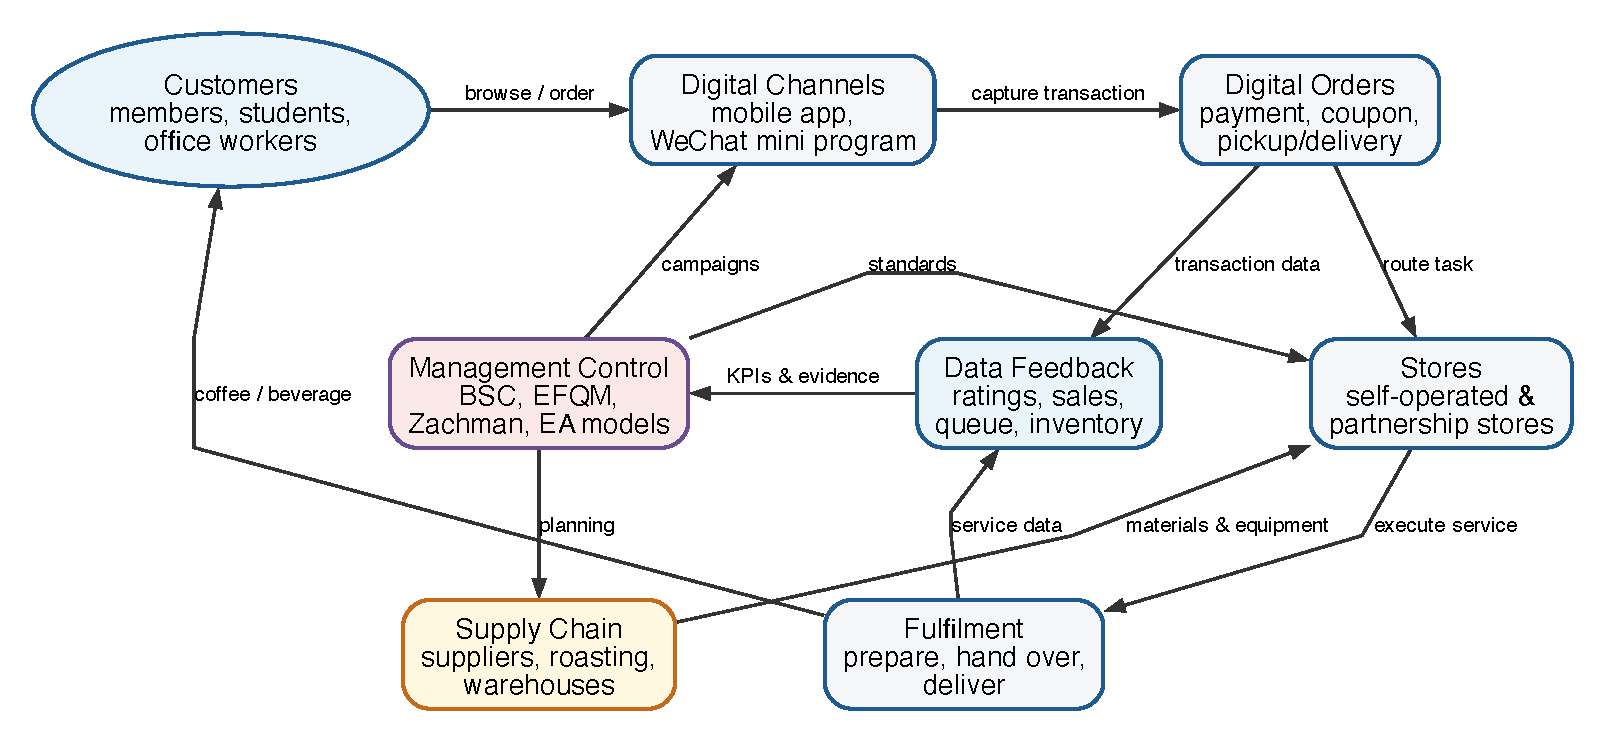
\includegraphics[width=0.95\textwidth]{integrated_operating_model.pdf}
\caption{Integrated operating model of Luckin Coffee used as the organizing logic for the Seminar 7 report.}
\label{fig:integrated}
\end{figure}

\subsection{Coverage of Seminar 7 Requirements}

\begin{table}[H]
\centering
\small
\caption{Traceability between the Seminar 7 instruction sheet and this report.}
\begin{tabularx}{\textwidth}{P{2.2cm}P{7.2cm}Y}
\toprule
\textbf{Item} & \textbf{Required content} & \textbf{Where covered} \\
\midrule
I--II & Title, business name, member names, group number & Title page and Section 1 \\
III & Background: products, services, mission, vision & Section 2 \\
IV & Business analysis: stakeholders, customers, financial, process, learning and growth & Section 3 \\
V & Balanced Scorecard with mission, objectives, measures & Section 4 \\
VI & Business Model Canvas & Section 5 \\
VII & EFQM nine criteria and related questions & Section 6 \\
VIII & Conceptual model & Section 7 \\
IX & First row of the Zachman Framework & Section 8 \\
X & Relational data model & Section 9 \\
XI & Business layer model mandatory; application and technology optional & Section 10 \\
XII & References & References section \\
\bottomrule
\end{tabularx}
\end{table}

% =================== BACKGROUND ===================
\section{Background of the Selected Business}

\subsection{Corporate Overview}

Luckin Coffee Inc. was founded in 2017 and is based in Xiamen, China. Its investor-relations materials describe the company as a pioneer of a ``technology-driven new retail model'' that provides coffee and other products with high quality, high affordability, and high convenience to customers~\cite{luckin_ir_overview}. The company sells freshly brewed coffee, tea-based beverages, non-coffee drinks, light food, packaged coffee products, and related retail products through a combination of self-operated stores, partnership stores, mobile channels, and delivery platforms.

Luckin's public mission is ``to create lucky moments and inspire,'' and its vision is ``to build a world-class coffee brand and become a part of everyone's daily life''~\cite{luckin_ir_overview}. These statements match its mass-market strategy: coffee and beverages are positioned as frequent, affordable, and convenient daily products rather than only as premium cafe experiences.

\subsection{Products and Services}

Luckin's products and services can be grouped into five categories:

\begin{itemize}[leftmargin=1.3em]
  \item \textbf{Freshly brewed coffee:} Americano, latte, cappuccino, coconut latte, flavored coffee, and seasonal coffee products.
  \item \textbf{Non-coffee beverages:} tea drinks, fruit beverages, light milk tea, and other freshly made drinks. In June 2026, Luckin reported that cumulative sales of non-coffee beverages had exceeded RMB 20 billion~\cite{luckin_noncoffee_2026}.
  \item \textbf{Food and complementary items:} light meals, snacks, desserts, and breakfast-related products.
  \item \textbf{Packaged coffee and retail products:} instant coffee, drip coffee, beans, capsules, and merchandise sold through online and offline channels.
  \item \textbf{Digital ordering and fulfilment service:} mobile app ordering, WeChat mini-program ordering, digital payment, coupon redemption, pickup, delivery, and order-status tracking.
\end{itemize}

\subsection{Scale and Current Snapshot}

Luckin's scale is central to its enterprise architecture. In FY2025, the company reported total net revenues of RMB 49.288 billion, 8,708 net new store openings, 31,048 total stores at year end, 94.2 million average monthly transacting customers, and GAAP operating income of RMB 5.073 billion~\cite{luckin_fy2025_results}. In Q1 2026, the store network further increased to 33,596 stores, including 21,807 self-operated stores and 11,789 partnership stores~\cite{luckin_q1_2026}. On June 8, 2026, the company stated that its global store network had exceeded 35,000 stores~\cite{luckin_noncoffee_2026}.

\begin{table}[H]
\centering
\caption{Business snapshot used in this report.}
\begin{tabularx}{\textwidth}{P{4.0cm}Y}
\toprule
\textbf{Dimension} & \textbf{Description} \\
\midrule
Business type & Technology-enabled coffee and beverage retail enterprise. \\
Core value proposition & Affordable, convenient, digitally ordered, and standardized coffee and beverage products. \\
Primary channels & Mobile app, WeChat mini-program, physical pickup stores, relax stores, delivery platforms, and e-commerce channels. \\
Store model & Combination of self-operated stores and partnership stores. \\
Strategic capability & Integration of customer data, store operations, supply chain, product innovation, and performance management. \\
Architecture relevance & The business depends on the alignment of strategy, process, data, applications, and technology infrastructure. \\
\bottomrule
\end{tabularx}
\end{table}

\begin{figure}[H]
  \centering
  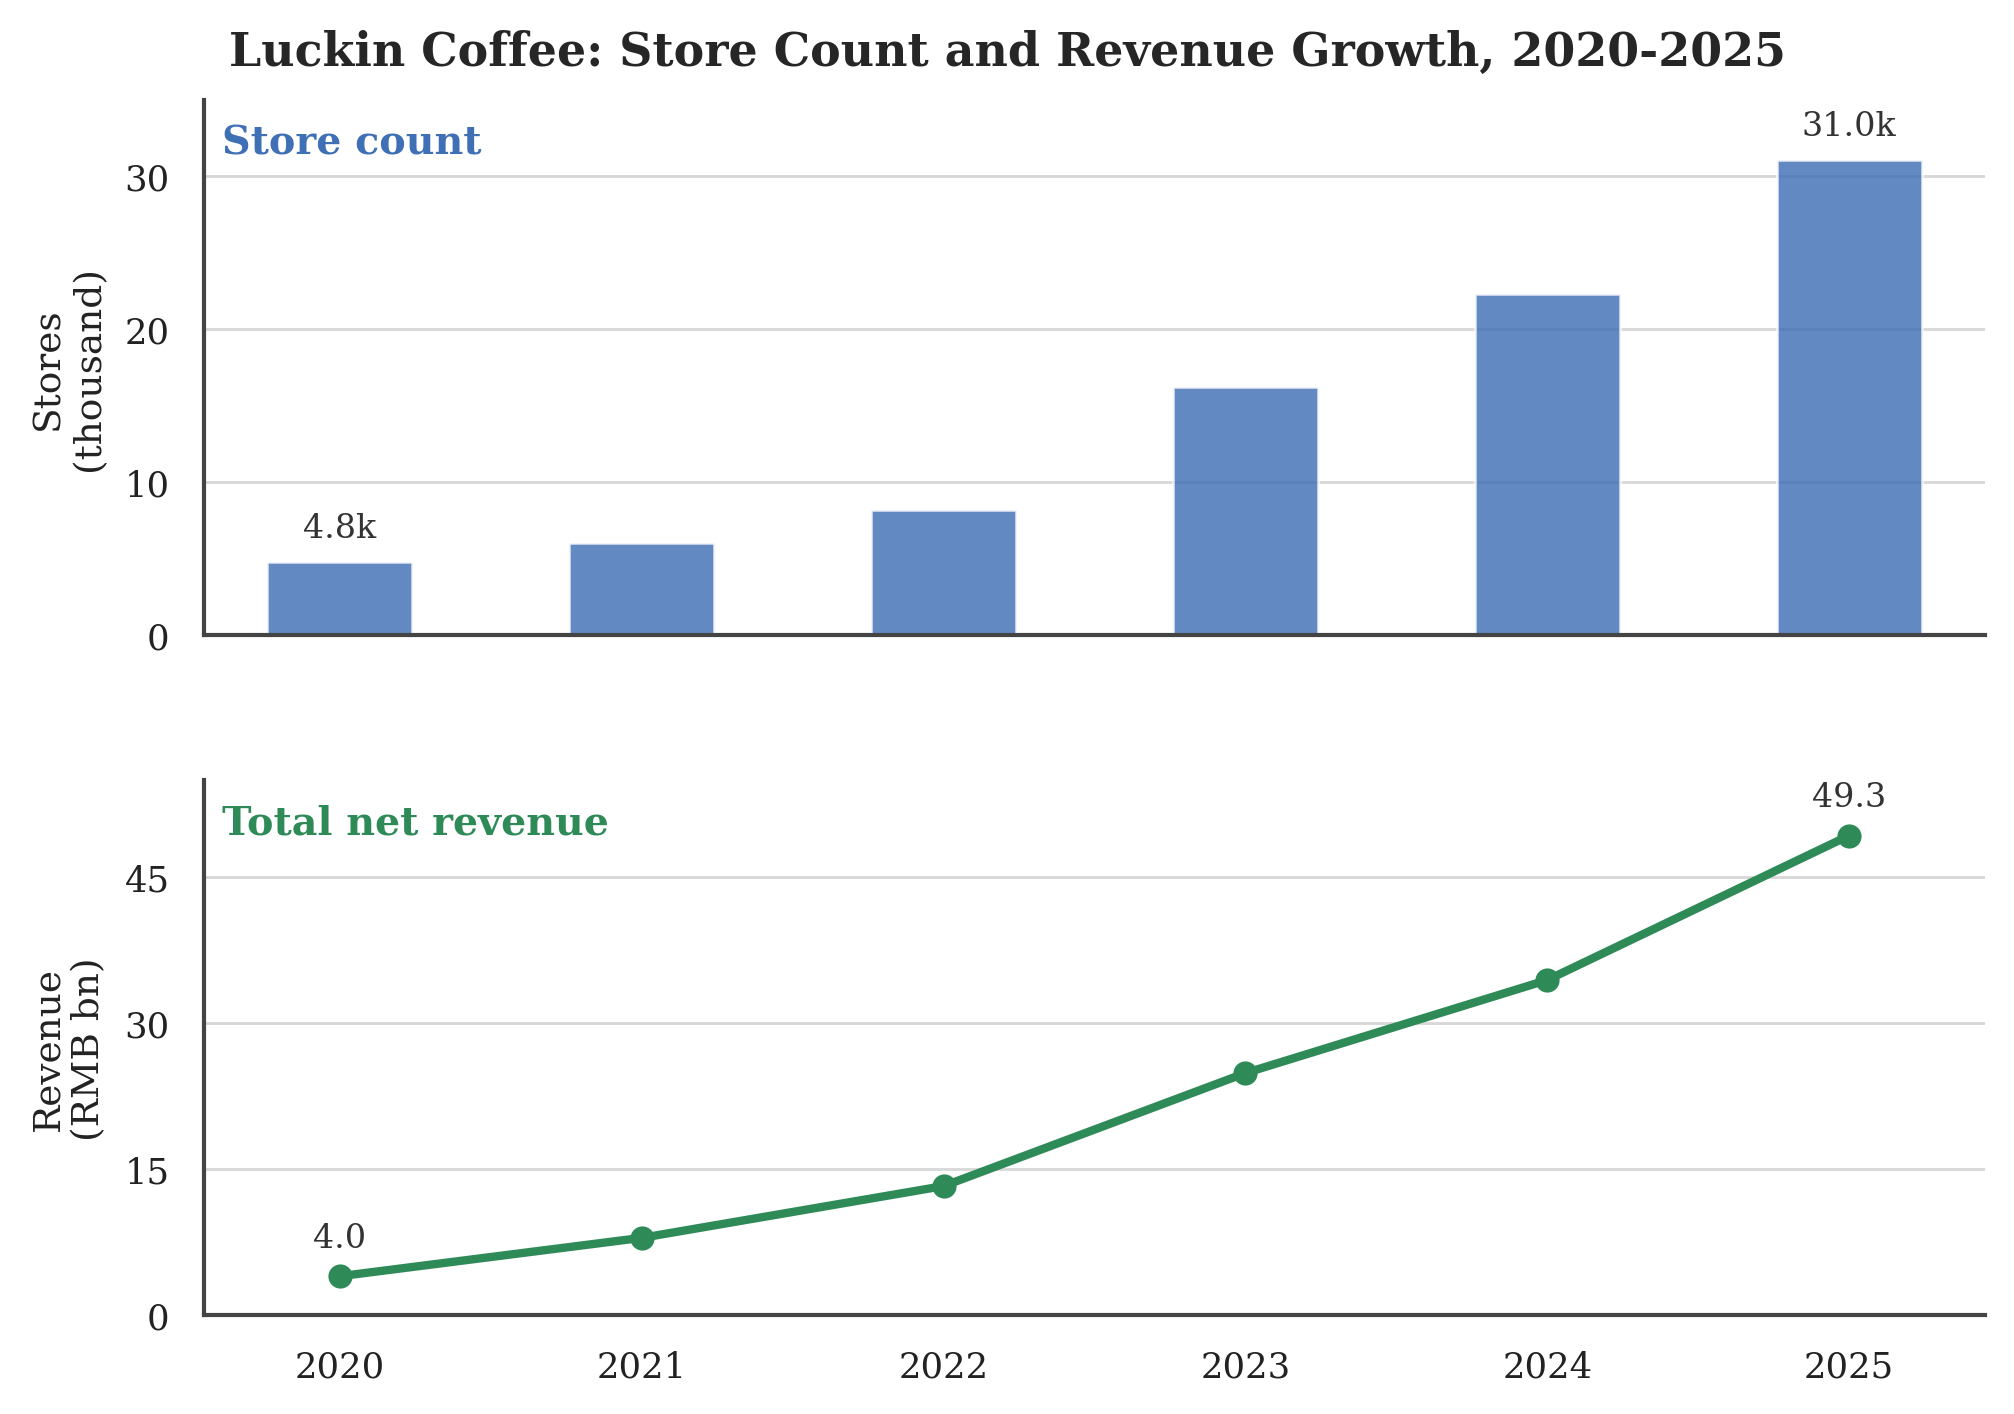
\includegraphics[width=0.82\textwidth]{fig_growth.png}
  \caption{Store-count and revenue-growth evidence drawn from the Seminar 1 case background analysis.}
\end{figure}

% =================== BUSINESS ANALYSIS ===================
\section{Business Analysis from Multiple Perspectives}

The business analysis follows five perspectives required by the Seminar 7 instruction sheet: stakeholders, customers, financial model, internal business processes, and learning and growth. Together they describe how Luckin creates, delivers, captures, and improves value.

\subsection{Stakeholders and Key Partners}

Luckin operates through a broad stakeholder ecosystem. The main stakeholders are customers, members, store employees, store managers, partnership-store operators, suppliers, logistics and delivery partners, payment platforms, landlords, investors, regulators, technology partners, and local communities.

\begin{figure}[H]
  \centering
  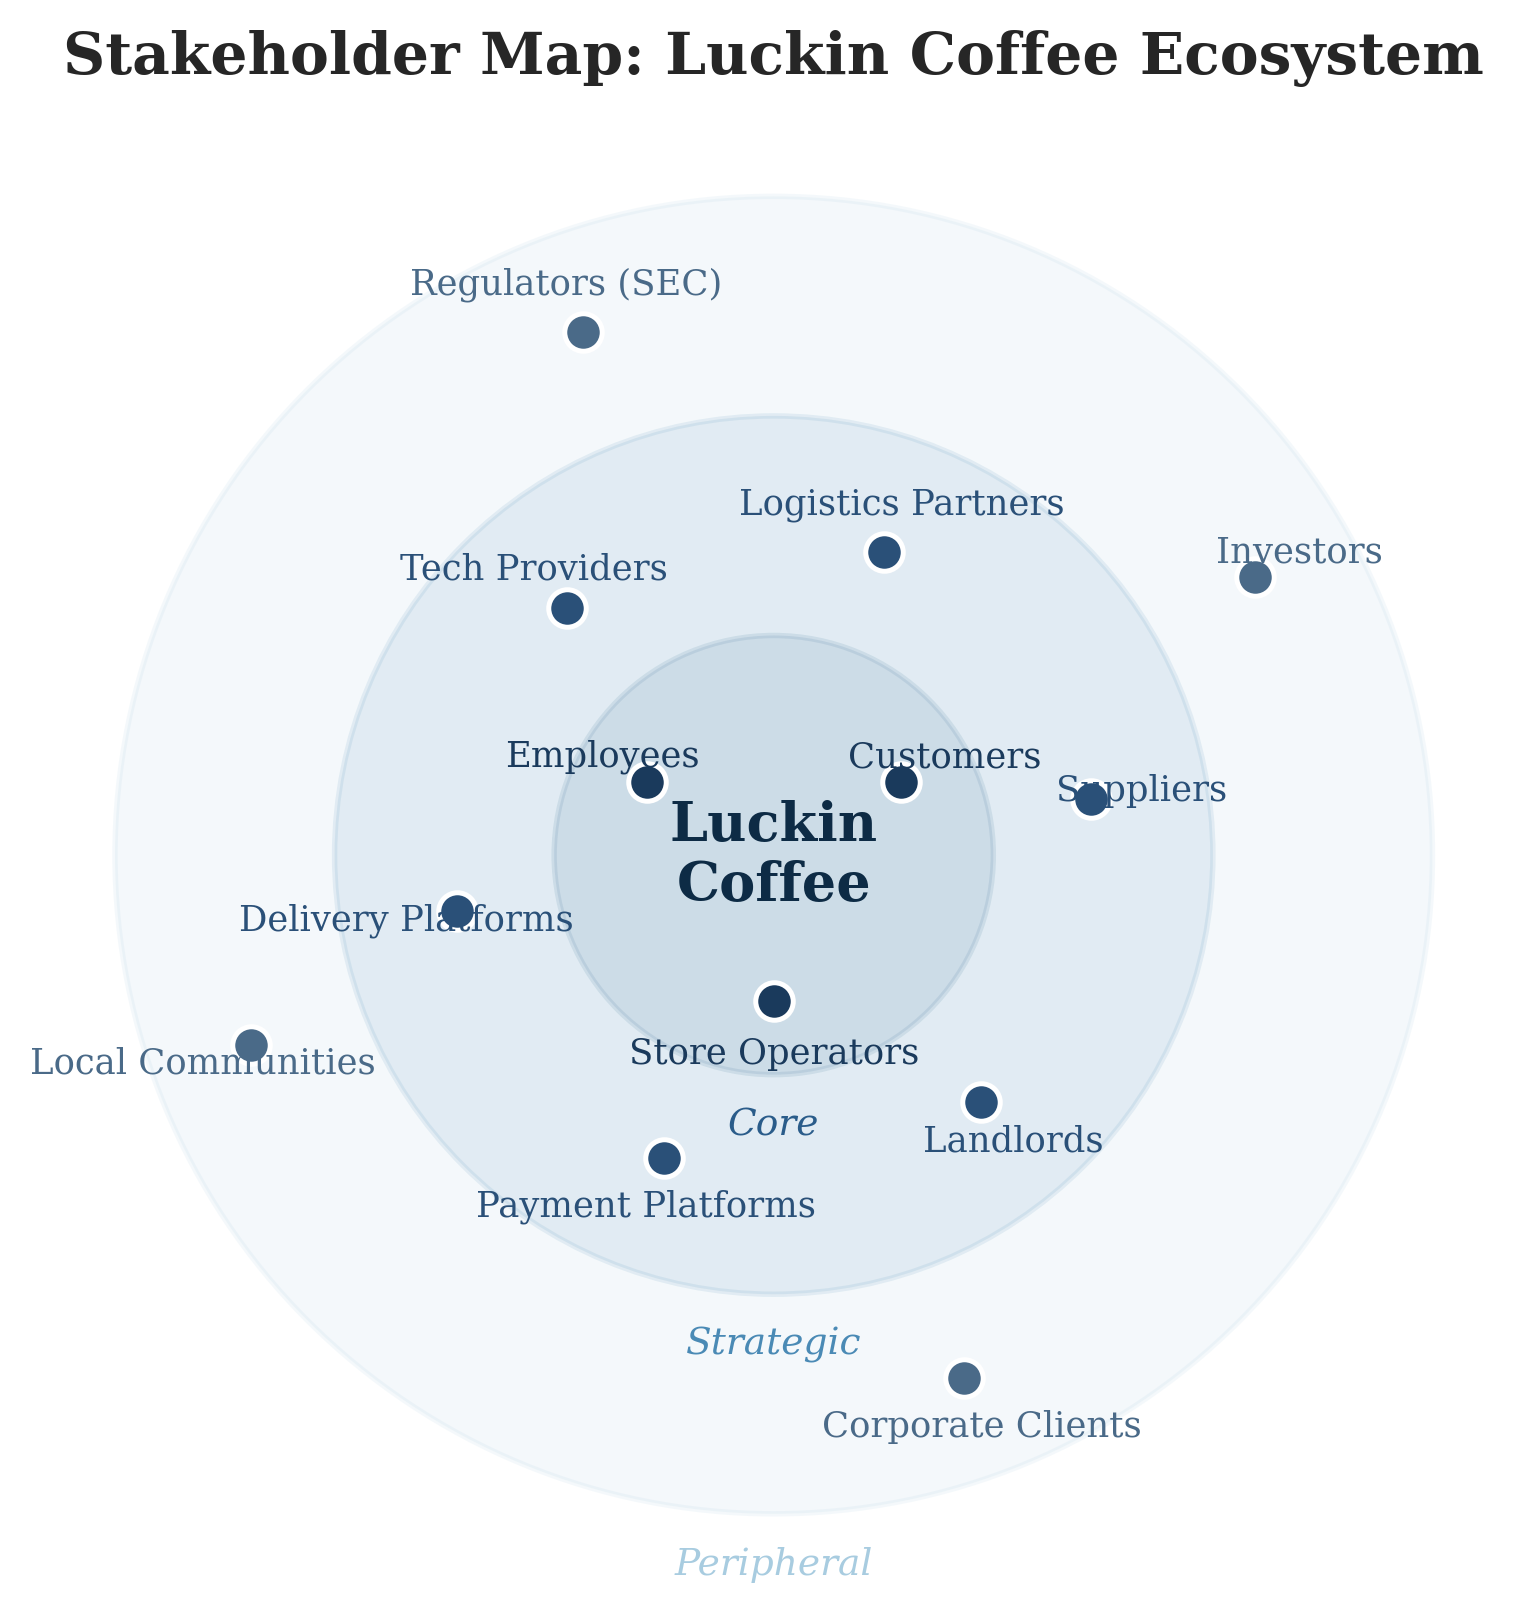
\includegraphics[width=0.82\textwidth]{fig_stakeholders.png}
  \caption{Stakeholder map adapted from the Seminar 1 analysis.}
\end{figure}

Key partners are especially important because Luckin's business model is not fully vertically owned. Coffee beans, dairy products, fruit ingredients, packaging materials, equipment, delivery capacity, payment interfaces, and digital ecosystem access all depend on partner relationships. At the same time, Luckin has strengthened its own supply-chain assets, including roasting centers and processing facilities, to improve product consistency and scalability~\cite{luckin_noncoffee_2026}.

\subsection{Customers, Relationships, and Channels}

Luckin targets mass-market urban consumers. Main customer types include office workers, students, commuters, price-sensitive young consumers, users who value coupons and convenience, and corporate or institutional buyers. These customer groups share a need for quick access, stable taste, digital payment, and predictable service.

The customer relationship is mainly digital. Customers browse products, receive coupons, place orders, pay, choose pickup or delivery, and submit feedback through digital interfaces. This relationship gives Luckin a direct data connection with customers, enabling personalized promotions, product testing, user segmentation, retention analysis, and customer lifetime value management.

\subsection{Financial Perspective}

Luckin makes money through two main streams: product sales from self-operated stores and revenue from partnership stores. Product sales include freshly brewed drinks, non-freshly brewed items, e-commerce, and delivery-related revenue. Partnership-store revenue includes materials sales, equipment sales, delivery service fees, profit sharing, royalty fees, franchise fees, and other services~\cite{luckin_fy2025_results,luckin_q1_2026}.

The major spending categories include material costs, store rent, labor, utilities, depreciation, delivery expenses, logistics, sales and marketing, general administration, technology development, and pre-opening expenses. FY2025 shows that Luckin had already reached large scale and positive operating income, but Q1 2026 also shows margin pressure from delivery expenses and competitive conditions~\cite{luckin_q1_2026}. Therefore, cost discipline and operational efficiency remain strategic priorities.

\subsection{Internal Business Process Perspective}

Luckin's core business process begins before the order and continues after fulfilment. Product teams develop and test new beverages. The supply chain sources and prepares ingredients. Digital channels publish menus and coupons. Customers place orders and make payment. The system routes each order to a store. Store staff prepare the drink according to recipe standards. Customers receive the product by pickup or delivery. Feedback and transaction data return to analytics and management dashboards.

\begin{figure}[H]
  \centering
  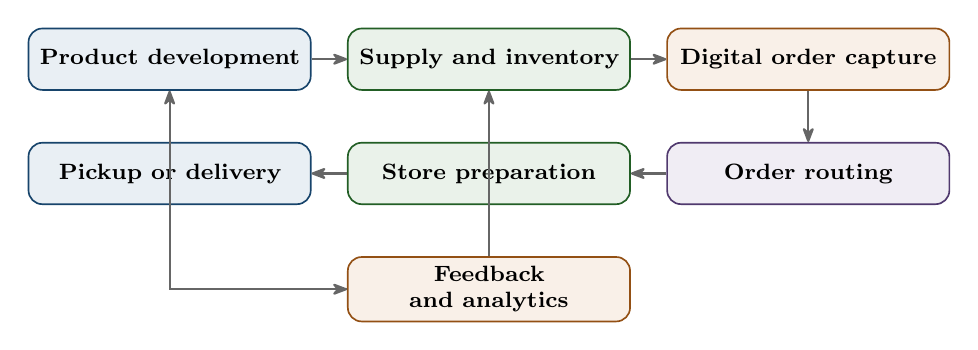
\begin{tikzpicture}[
    node distance=0.9cm,
    box/.style={rectangle, rounded corners=5pt, draw=#1!75!black, fill=#1!10,
                text width=3.35cm, minimum height=0.78cm, align=center,
                font=\footnotesize\bfseries, line width=0.6pt},
    arrow/.style={-{Stealth[round]}, line width=0.8pt, black!60}
  ]
    \node[box=lkblue] (dev) {Product development};
    \node[box=lkgreen, right=0.45cm of dev] (supply) {Supply and inventory};
    \node[box=lkorange, right=0.45cm of supply] (order) {Digital order capture};
    \node[box=lkpurple, below=0.65cm of order] (route) {Order routing};
    \node[box=lkgreen, left=0.45cm of route] (store) {Store preparation};
    \node[box=lkblue, left=0.45cm of store] (handover) {Pickup or delivery};
    \node[box=lkorange, below=0.65cm of store] (data) {Feedback and analytics};

    \draw[arrow] (dev) -- (supply);
    \draw[arrow] (supply) -- (order);
    \draw[arrow] (order) -- (route);
    \draw[arrow] (route) -- (store);
    \draw[arrow] (store) -- (handover);
    \draw[arrow] (handover) |- (data);
    \draw[arrow] (data) -| (dev);
    \draw[arrow] (data) -- (supply);
  \end{tikzpicture}
  \caption{Closed-loop business process for Luckin Coffee.}
\end{figure}

\subsection{Learning and Growth Perspective}

Luckin's learning and growth capability comes from product innovation, digital operations, standardized employee training, supply-chain strengthening, and data-based management. Customer data supports product testing and targeted promotions. Store data supports staffing and productivity management. Inventory data supports replenishment and waste reduction. Training systems support consistency across thousands of stores.

The main risk is that rapid expansion may create pressure on quality control, employee experience, partnership-store consistency, data governance, and brand trust. Therefore, long-term learning should include not only sales growth but also risk management, compliance, employee development, social responsibility, and system resilience.

% =================== BSC ===================
\section{Balanced Scorecard}

The Balanced Scorecard translates Luckin's strategy into missions, objectives, and measures across four perspectives: financial, customer, internal process, and learning and growth.

\begin{figure}[H]
  \centering
  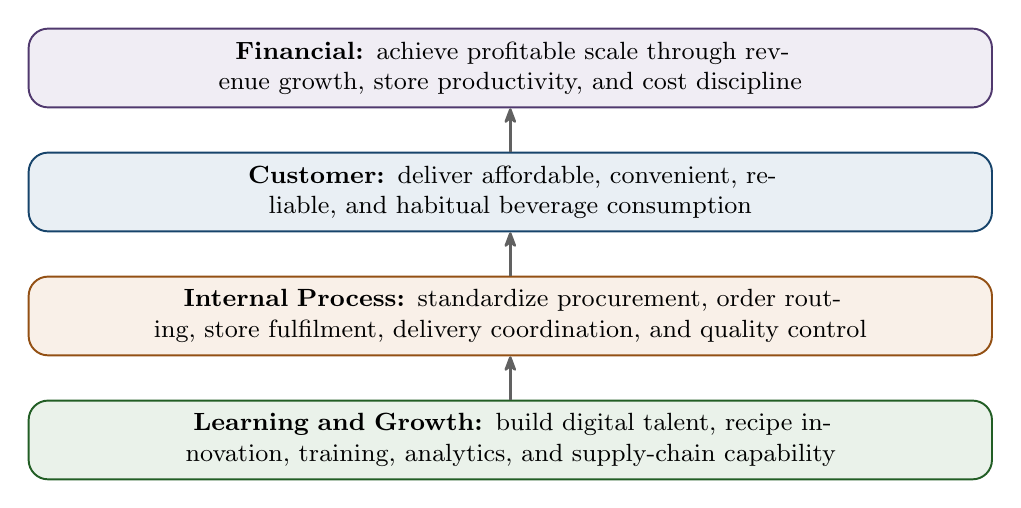
\begin{tikzpicture}[
    layer/.style={rectangle, rounded corners=7pt, draw=#1!75!black, fill=#1!10,
                  text width=12.0cm, minimum height=1.0cm, align=center,
                  font=\small, line width=0.7pt},
    arrow/.style={-{Stealth[round]}, line width=0.9pt, black!62}
  ]
    \node[layer=lkgreen] (lg) {\textbf{Learning and Growth:} build digital talent, recipe innovation, training, analytics, and supply-chain capability};
    \node[layer=lkorange, above=0.55cm of lg] (ip) {\textbf{Internal Process:} standardize procurement, order routing, store fulfilment, delivery coordination, and quality control};
    \node[layer=lkblue, above=0.55cm of ip] (cu) {\textbf{Customer:} deliver affordable, convenient, reliable, and habitual beverage consumption};
    \node[layer=lkpurple, above=0.55cm of cu] (fi) {\textbf{Financial:} achieve profitable scale through revenue growth, store productivity, and cost discipline};
    \draw[arrow] (lg) -- (ip);
    \draw[arrow] (ip) -- (cu);
    \draw[arrow] (cu) -- (fi);
  \end{tikzpicture}
  \caption{Balanced Scorecard strategy map for Luckin Coffee.}
\end{figure}

\begin{landscape}
\thispagestyle{empty}
\begin{table}[H]
\centering
\scriptsize
\renewcommand{\arraystretch}{1.12}
\caption{Balanced Scorecard table for Luckin Coffee.}
\begin{tabularx}{\linewidth}{P{2.8cm}P{5.1cm}P{8.0cm}Y}
\toprule
\textbf{Perspective} & \textbf{Mission} & \textbf{Objectives} & \textbf{Measures} \\
\midrule
\textbf{Financial} &
Build a scalable and profitable coffee and beverage retail platform while keeping products affordable. &
\begin{enumerate}[leftmargin=*,nosep]
  \item Increase total net revenue through store expansion, customer frequency, and product diversification.
  \item Improve store-level profitability through self-operated efficiency and partnership-store scale.
  \item Control cost pressure from materials, rent, labor, logistics, delivery, and marketing.
\end{enumerate} &
\begin{enumerate}[leftmargin=*,nosep]
  \item Total net revenue, revenue growth, GMV, same-store sales growth.
  \item Store-level operating margin, average order value, revenue per store, partnership-store revenue.
  \item Material cost ratio, rent and labor cost ratio, delivery cost per order, promotion expense ratio.
\end{enumerate} \\
\midrule
\textbf{Customer} &
Make Luckin a convenient, affordable, and reliable part of customers' daily beverage routines. &
\begin{enumerate}[leftmargin=*,nosep]
  \item Increase retention, repeat purchase, and membership engagement.
  \item Improve convenience through fast pickup, reliable delivery, and dense store coverage.
  \item Strengthen brand trust through taste consistency, hygiene, and complaint handling.
\end{enumerate} &
\begin{enumerate}[leftmargin=*,nosep]
  \item Average monthly transacting customers, active members, repeat purchase rate, customer lifetime value.
  \item Average pickup time, delivery completion time, nearby-store coverage, cancellation rate.
  \item Customer rating, complaint rate, quality complaint rate, net promoter score.
\end{enumerate} \\
\midrule
\textbf{Internal Process} &
Operate an integrated digital-to-physical value chain from demand forecasting to store fulfilment. &
\begin{enumerate}[leftmargin=*,nosep]
  \item Standardize procurement, recipe execution, production, fulfilment, and quality control.
  \item Use data systems to improve forecasting, inventory, replenishment, and scheduling.
  \item Reduce friction in app ordering, payment, routing, preparation, and after-sales feedback.
\end{enumerate} &
\begin{enumerate}[leftmargin=*,nosep]
  \item Recipe compliance rate, store audit pass rate, order accuracy, product consistency indicators.
  \item Forecast accuracy, inventory turnover, stockout rate, wastage rate, labor utilization.
  \item System uptime, transaction success rate, routing error rate, feedback response time.
\end{enumerate} \\
\midrule
\textbf{Learning and Growth} &
Develop the people, data, technology, and innovation capabilities needed for sustainable expansion. &
\begin{enumerate}[leftmargin=*,nosep]
  \item Improve employee training, store-manager capability, and partnership-store execution.
  \item Accelerate product innovation while maintaining quality and margin discipline.
  \item Strengthen data governance, compliance, and infrastructure resilience.
\end{enumerate} &
\begin{enumerate}[leftmargin=*,nosep]
  \item Training completion rate, employee productivity, turnover, engagement, safety incidents.
  \item New-product contribution, product launch success rate, defect rate, gross-margin change.
  \item Data-quality score, incident recovery time, compliance audit results, system availability.
\end{enumerate} \\
\bottomrule
\end{tabularx}
\end{table}
\end{landscape}

% =================== BMC ===================
\clearpage
\begin{landscape}
\thispagestyle{empty}
\section{Business Model Canvas}

The Business Model Canvas summarizes how Luckin creates value, delivers value to customers, and captures financial returns.

\begin{table}[H]
\portraitlandscapepagenumber
\centering
\footnotesize
\setlength{\tabcolsep}{3.5pt}
\renewcommand{\arraystretch}{1.18}
\caption{Business Model Canvas for Luckin Coffee.}
\begin{tabular}{|P{4.55cm}|P{4.55cm}|P{4.55cm}|P{4.55cm}|P{4.55cm}|}
\hline
\textbf{Key Partners} &
\textbf{Key Activities} &
\textbf{Value Propositions} &
\textbf{Customer Relationships} &
\textbf{Customer Segments} \\
\hline
Coffee-bean suppliers, dairy and ingredient suppliers, packaging suppliers, equipment vendors, delivery partners, payment platforms, landlords, partnership-store operators, technology vendors. &
Product development, menu management, digital ordering, coupon campaigns, store fulfilment, quality control, inventory replenishment, delivery coordination, data analytics, partner management. &
Affordable and convenient coffee and beverages; mobile-first purchase journey; fast pickup and delivery; stable taste through standardized recipes; frequent product innovation; dense store coverage. &
Digital membership, app and WeChat interaction, personalized coupons, push notifications, order-status tracking, customer feedback, complaint handling, loyalty programs. &
Office workers, students, young urban consumers, commuters, coupon-sensitive consumers, coffee and non-coffee beverage buyers, corporate and group buyers. \\
\hline
\multicolumn{2}{|P{9.31cm}|}{\textbf{Key Resources}

Brand, mobile app and mini-program, data platform, store network, trained staff, recipe standards, roasting and processing capabilities, suppliers, partnership-store network, customer data, operational dashboards.} &
\textbf{Channels}

Mobile app, WeChat mini-program, pickup stores, relax stores, delivery platforms, e-commerce stores, social media, corporate purchasing channels. &
\multicolumn{2}{P{9.31cm}|}{\textbf{Cost Structure}

Materials, packaging, store rent, labor, utilities, equipment depreciation, delivery expenses, logistics, marketing, platform commissions, technology development, administration, training, quality management.} \\
\hline
\multicolumn{5}{|P{23.88cm}|}{\textbf{Revenue Streams}

Self-operated store product sales, freshly brewed drink sales, other products, e-commerce sales, delivery fees, partnership-store material sales, equipment sales, profit sharing, royalties, franchise and service fees.} \\
\hline
\end{tabular}
\end{table}
\end{landscape}
\clearpage

% =================== EFQM ===================
\section{EFQM Excellence Model Evaluation}

EFQM is a quality-management approach that evaluates an organization through enablers and results. For Luckin, the model helps connect strategic ambition with daily execution and measurable outcomes. This report applies the classic nine-criterion EFQM Excellence Model as required by the seminar instruction.

\begin{figure}[H]
  \centering
  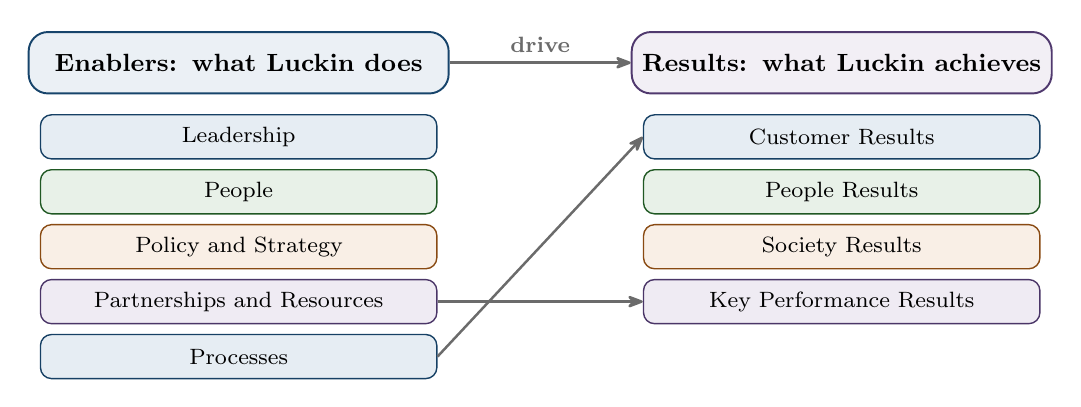
\begin{tikzpicture}[
    node distance=0.75cm,
    group/.style={rectangle, rounded corners=7pt, draw=#1!75!black, fill=#1!9,
                  text width=5.1cm, minimum height=0.78cm, align=center,
                  font=\small\bfseries, line width=0.7pt},
    item/.style={rectangle, rounded corners=4pt, draw=#1!70!black, fill=#1!11,
                  text width=4.8cm, minimum height=0.56cm, align=center,
                  font=\footnotesize, line width=0.5pt},
    arrow/.style={-{Stealth[round]}, line width=0.9pt, black!58}
  ]
    \node[group=lkblue] (enablers) {Enablers: what Luckin does};
    \node[item=lkblue, below=0.25cm of enablers] (lead) {Leadership};
    \node[item=lkgreen, below=0.12cm of lead] (people) {People};
    \node[item=lkorange, below=0.12cm of people] (strategy) {Policy and Strategy};
    \node[item=lkpurple, below=0.12cm of strategy] (resources) {Partnerships and Resources};
    \node[item=lkblue, below=0.12cm of resources] (processes) {Processes};
    \node[group=lkpurple, right=2.3cm of enablers] (results) {Results: what Luckin achieves};
    \node[item=lkblue, below=0.25cm of results] (cust) {Customer Results};
    \node[item=lkgreen, below=0.12cm of cust] (pres) {People Results};
    \node[item=lkorange, below=0.12cm of pres] (soc) {Society Results};
    \node[item=lkpurple, below=0.12cm of soc] (key) {Key Performance Results};
    \draw[arrow] (enablers) -- node[above, font=\footnotesize\bfseries] {drive} (results);
    \draw[arrow] (processes.east) -- (cust.west);
    \draw[arrow] (resources.east) -- (key.west);
  \end{tikzpicture}
  \caption{EFQM logic applied to Luckin Coffee.}
\end{figure}

\begin{longtable}{P{2.65cm}P{5.45cm}P{5.95cm}}
\caption{EFQM nine-criterion evaluation for Luckin Coffee.}\\
\toprule
\textbf{Criterion} & \textbf{Answers to the required questions} & \textbf{Evaluation and improvement focus} \\
\midrule
\endfirsthead
\toprule
\textbf{Criterion} & \textbf{Answers to the required questions} & \textbf{Evaluation and improvement focus} \\
\midrule
\endhead
\bottomrule
\endlastfoot
\textbf{Leadership} &
Leaders include the board, CEO, executive team, regional managers, product leaders, technology leaders, and store-management teams. They define the vision, set growth priorities, review performance, communicate standards, and connect digital strategy with store execution. Leadership is practiced through mission communication, operating dashboards, compliance controls, and performance reviews. &
Strong in strategic execution and data-based control. Improvement should focus on long-term trust, transparent governance, risk oversight, and avoiding an overly narrow focus on growth speed. \\
\midrule
\textbf{People} &
People include store staff, store managers, product teams, technology teams, supply-chain staff, corporate managers, and partner-store operators. They are managed through SOPs, training modules, scheduling, performance indicators, and store audits. Involvement occurs through operational feedback, service improvement, and training. &
Good at standardization and training. Improvement should include employee engagement, retention, career development, safety, and balance between productivity metrics and human well-being. \\
\midrule
\textbf{Policy and Strategy} &
Stakeholders are identified through customer data, investor disclosures, partner management, supplier relationships, regulatory duties, and community impact. Future direction is informed by transaction data, store performance, supply-chain data, market competition, consumer trends, and financial reporting. Plans are implemented through systems, dashboards, recipes, campaigns, and store routines. &
Very strong in embedding strategy into digital operations. Improvement should make sustainability, data ethics, partnership-store quality, and brand-trust goals more measurable. \\
\midrule
\textbf{Partnerships and Resources} &
Partnerships are cooperative relationships that provide capabilities Luckin does not fully own, such as ingredients, delivery capacity, store operation, payment, and technology support. Good partners should improve reliability, quality, scale, cost, and customer experience. Resources include finance, stores, equipment, staff, recipes, raw materials, data, technology, information, and knowledge. &
Strong because the model combines owned capabilities with external scale. Improvement should reduce dependency risks, strengthen supplier audits, and ensure consistent partner-store execution. \\
\midrule
\textbf{Processes} &
Processes are repeated activities that transform inputs into customer value. Key processes include product development, procurement, campaign management, order capture, payment, order routing, store preparation, delivery/pickup, customer feedback, replenishment, and performance review. Processes are managed by SOPs, systems, data dashboards, and audits. &
Very strong. Luckin's competitive advantage depends on process standardization and digital coordination. Improvement should focus on system resilience, exception handling, data quality, and cross-store consistency. \\
\midrule
\textbf{Customer Results} &
Customer results are important because convenience, affordability, taste, and trust directly determine repeat purchases. Luckin should measure perception indicators such as satisfaction, app rating, complaint themes, and brand trust, plus performance indicators such as pickup time, delivery time, cancellation rate, retention, and repeat purchase. Results should be communicated through dashboards and visual reports. &
Strong because customer behavior is highly measurable. Improvement should distinguish promotion-driven purchases from long-term loyalty and monitor quality consistency across store types. \\
\midrule
\textbf{People Results} &
People results measure whether employee management supports business excellence. Luckin should report training completion, SOP pass rate, productivity, turnover, engagement, safety incidents, career progression, and store-manager capability. Results should be communicated to managers and used to adjust training and scheduling. &
Moderate to strong. Operational productivity is measurable, but softer people outcomes need more explicit measurement. \\
\midrule
\textbf{Society Results} &
Society results matter because a large retail chain affects communities, suppliers, farmers, consumers, data privacy, and public trust. Luckin should report sustainability initiatives, responsible sourcing, local agricultural support, waste reduction, governance reform, and data responsibility. Communication can use ESG reports, annual reports, public announcements, and local community materials. &
Developing. The company has clear opportunities to strengthen social-value reporting, responsible sourcing targets, waste metrics, and privacy governance. \\
\midrule
\textbf{Key Performance Results} &
Key performance results are the financial and non-financial outcomes that show whether the strategy works. The range includes revenue, operating income, store count, customer base, store-level margin, product sales, inventory, delivery cost, system uptime, and campaign effectiveness. Results should be measured through reliable data collection, regular reporting, and benchmarking. &
Strong in scale and financial disclosure. Improvement should build a culture where measurement drives learning, not only short-term targets. \\
\end{longtable}

% =================== CONCEPTUAL MODEL ===================
\section{Conceptual Model}

The conceptual model describes the business objects and relationships behind Luckin's mobile-first retail system. It is independent of implementation details, but it provides the basis for the relational data model and the application architecture.

\begin{landscape}
\thispagestyle{empty}
\begin{center}
\captionsetup{hypcap=false}
\captionof{figure}{Conceptual model of Luckin Coffee's mobile-first retail operating system.}
\vspace{0.2cm}
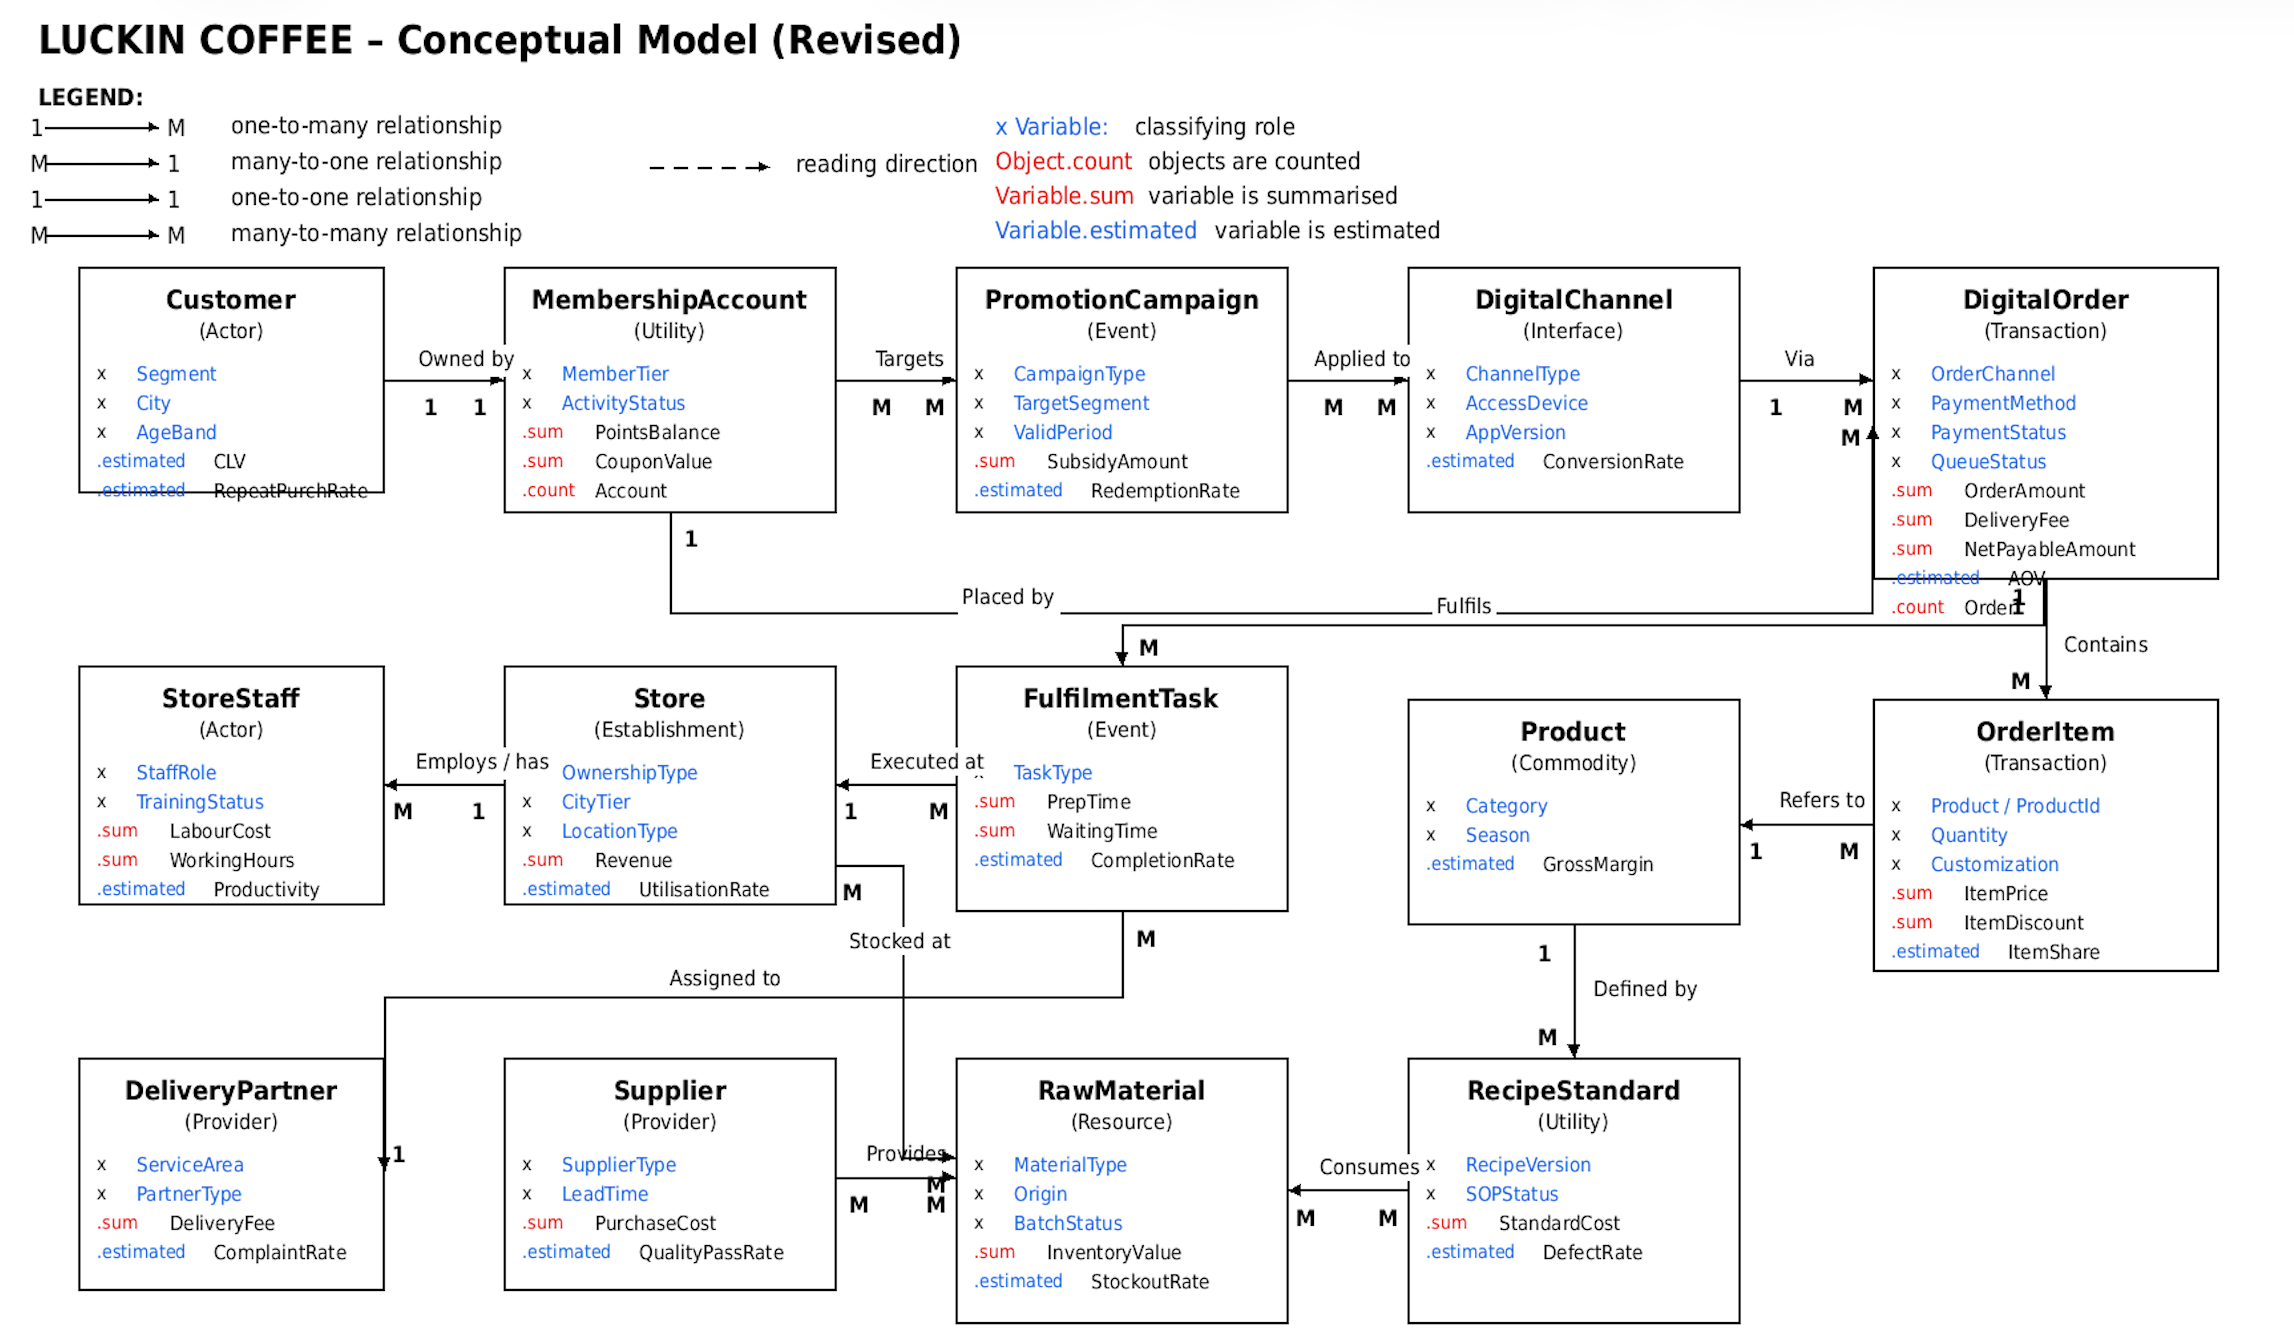
\includegraphics[width=0.98\linewidth,height=14.0cm,keepaspectratio]{conceptual_model_original.png}
\end{center}
\end{landscape}

\begin{table}[H]
\centering
\small
\caption{Main conceptual objects and business meaning.}
\begin{tabularx}{\textwidth}{P{3.6cm}Y}
\toprule
\textbf{Object group} & \textbf{Business meaning} \\
\midrule
Customer and membership & Identifies customer segments, member accounts, points, coupons, preferences, and repeat-purchase behavior. \\
Digital channel and order & Captures the transaction through app, mini-program, payment, order status, pickup, or delivery. \\
Product and recipe & Separates what customers buy from the standardized recipes and SOPs used to produce it. \\
Store and staff & Represents the physical fulfilment unit, ownership type, location type, staff roles, training, and productivity. \\
Supplier and material & Represents ingredients, origins, batches, supplier lead time, inventory value, and material quality. \\
Fulfilment and delivery & Represents preparation, waiting time, delivery support, completion, exception handling, and customer feedback. \\
Performance analytics & Converts operational data into KPIs such as AOV, margin, conversion rate, stockout rate, complaint rate, and CLV. \\
\bottomrule
\end{tabularx}
\end{table}

The model shows why Luckin's architecture needs both transactional data and analytical data. A digital order is not only a sales record; it also generates operational evidence about customer demand, coupon effectiveness, store workload, product performance, and supply-chain planning.

% =================== ZACHMAN ===================
\section{Zachman Framework: First Row}

The first row of the Zachman Framework is the contextual or planner view. It defines the enterprise scope by answering What, How, Where, Who, When, and Why at a high level.

\begin{landscape}
\thispagestyle{empty}
\begin{table}[H]
\portraitlandscapepagenumber
\centering
\scriptsize
\renewcommand{\arraystretch}{1.15}
\caption{Zachman Framework Row 1 for Luckin Coffee.}
\begin{tabularx}{\linewidth}{P{2.2cm} *{6}{Y}}
\toprule
& \textbf{Data} \newline What? & \textbf{Function} \newline How? & \textbf{Network} \newline Where? & \textbf{People} \newline Who? & \textbf{Time} \newline When? & \textbf{Motivation} \newline Why? \\
\midrule
\textbf{Scope / Contextual / Planner} &
Customers, members, channels, orders, products, recipes, stores, staff, suppliers, materials, delivery partners, campaigns, KPIs. &
Attract customers, publish menu, issue coupons, capture orders, confirm payment, prepare products, deliver or hand over, replenish materials, analyze results. &
Mobile app, WeChat mini-program, cloud systems, headquarters, self-operated stores, partnership stores, warehouses, supplier origins, delivery areas. &
Customers, members, baristas, store managers, franchise partners, suppliers, delivery riders, product teams, IT teams, finance teams, regulators, investors. &
App sessions, campaign periods, order time, payment time, queue status, store opening hours, peak demand, replenishment cycles, recipe effective dates. &
Affordable convenience, product quality, fast fulfilment, profitable scale, customer loyalty, data-driven improvement, supply reliability, brand trust. \\
\bottomrule
\end{tabularx}
\end{table}
\end{landscape}

This first row ensures that later models do not become isolated technical diagrams. The data model must represent the business things, the process model must represent the functions, the application layer must support the channels, and the performance system must reflect the motivations.

% =================== RELATIONAL DATA MODEL ===================
\section{Relational Data Model}

The relational data model transforms the conceptual model into implementable database relations. Each main object becomes a table, one-to-many relationships are represented through foreign keys, and many-to-many relationships are resolved through bridge tables.

\begin{figure}[H]
\centering
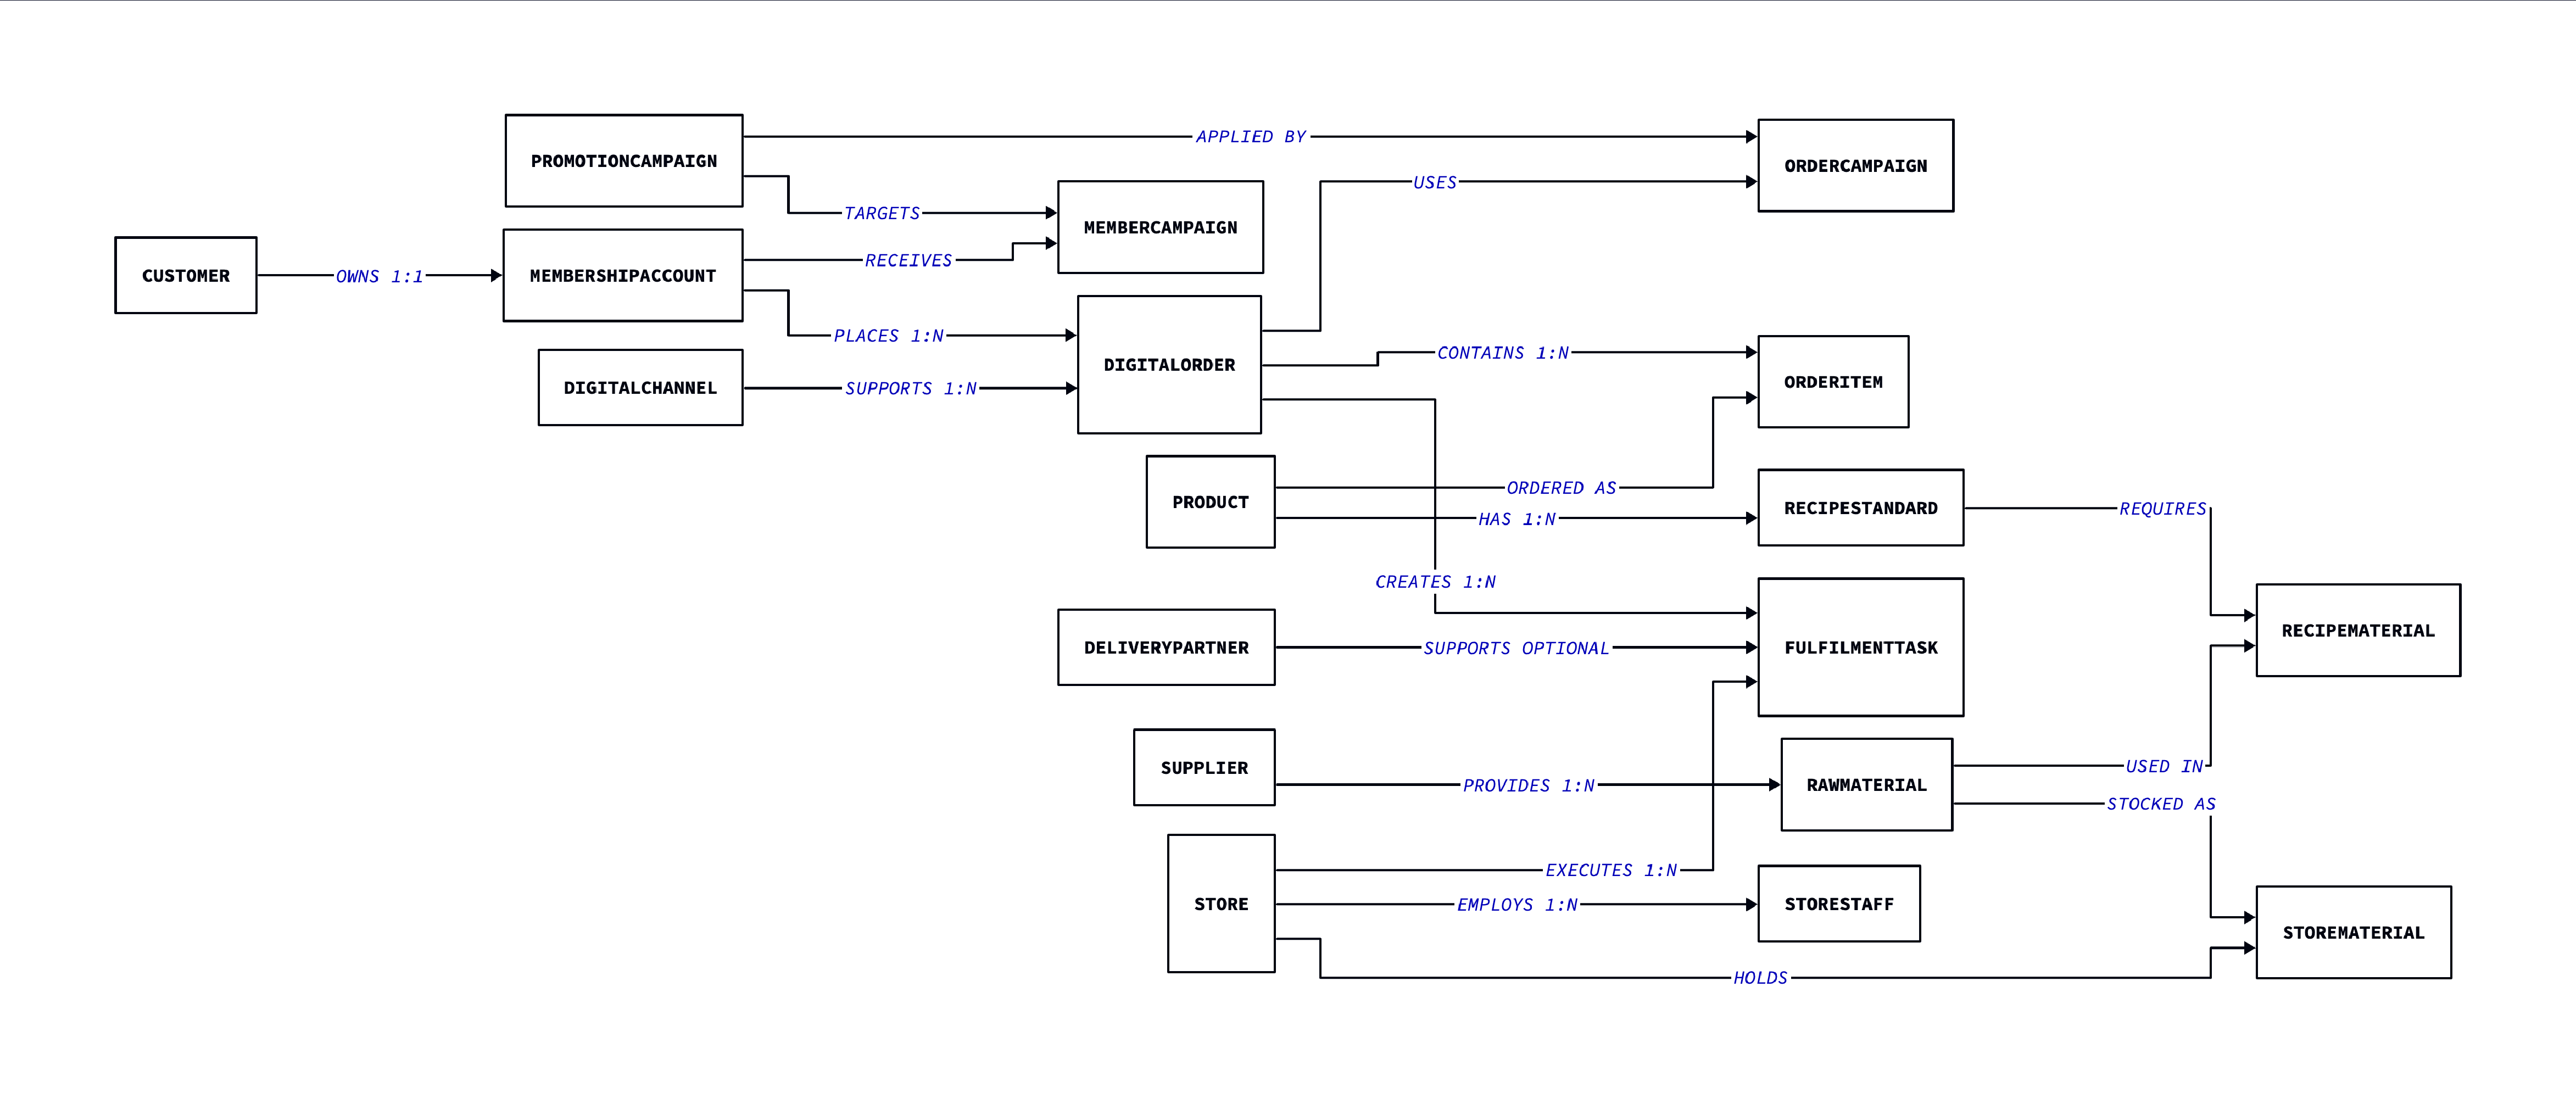
\includegraphics[width=\textwidth]{data_model_summary.pdf}
\caption{Summary of major relationships in the relational data model.}
\end{figure}

\scriptsize
\begin{longtable}{P{3.1cm}P{11.35cm}}
\caption{Relational data model transformed from the conceptual model.}\\
\toprule
\textbf{Relation} & \textbf{Attributes} \\
\midrule
\endfirsthead
\toprule
\textbf{Relation} & \textbf{Attributes} \\
\midrule
\endhead
\bottomrule
\endlastfoot
Customers & \pk{CustomerId}, Segment, City, AgeBand \\
MembershipAccounts & \pk{MemberId}, CustomerId\fk~(Unique), PointsBalance, CouponValue, MemberTier, ActivityStatus \\
DigitalChannels & \pk{ChannelId}, ChannelType, AccessDevice, AppVersion \\
PromotionCampaigns & \pk{CampaignId}, CampaignType, TargetSegment, StartDate, EndDate, SubsidyAmount \\
MemberCampaigns & \pk{MemberId}\pkfk, \pk{CampaignId}\pkfk, ReceivedDate, UsedStatus \\
DigitalOrders & \pk{OrderId}, MemberId\fk, ChannelId\fk, PaymentMethod, QueueStatus, GrossOrderAmount, CampaignDiscountAmount, ItemDiscountAmount, ActualDeliveryFee, NetPayableAmount, OrderDate, OrderTime \\
OrderCampaigns & \pk{OrderId}\pkfk, \pk{CampaignId}\pkfk, AppliedAmount \\
Products & \pk{ProductId}, ProductName, Category, Season, GrossMargin, CurrentStandardCost \\
OrderItems & \pk{OrderId}\pkfk, \pk{ItemNr}, ProductId\fk, Quantity, Customization, LineDiscountAmount, UnitItemPrice \\
DeliveryPartners & \pk{PartnerId}, PartnerName, PartnerType, ServiceArea, StandardDeliveryFee, ComplaintRate \\
Stores & \pk{StoreId}, StoreName, OwnershipType, CityTier, LocationType, Revenue, LaborCost \\
FulfilmentTasks & \pk{TaskId}, OrderId\fk, StoreId\fk, PartnerId\fk\nullable, TaskType, PrepTime, WaitingTime, CompletionRate, Status \\
StoreStaff & \pk{StaffId}, StoreId\fk, StaffName, StaffRole, TrainingStatus, WorkingHours, LaborCost, Productivity \\
Suppliers & \pk{SupplierId}, SupplierName, SupplierType, LeadTime \\
RawMaterials & \pk{MaterialId}, SupplierId\fk, MaterialName, MaterialType, Origin, BatchStatus, InventoryValue \\
StoreMaterials & \pk{StoreId}\pkfk, \pk{MaterialId}\pkfk, StockLevel, StockoutRate \\
RecipeStandards & \pk{RecipeId}, ProductId\fk, RecipeVersion, SopStatus, RecipeStandardCost, DefectRate, EffectiveFrom, EffectiveTo \\
RecipeMaterials & \pk{RecipeId}\pkfk, \pk{MaterialId}\pkfk, DosageAmount, DosageUnit \\
\end{longtable}
\normalsize

\begin{table}[H]
\centering
\small
\caption{Important integrity rules for the data model.}
\begin{tabularx}{\textwidth}{P{4.0cm}Y}
\toprule
\textbf{Rule type} & \textbf{Rule} \\
\midrule
Entity integrity & Every relation has a primary key; key values cannot be null. \\
Referential integrity & Foreign keys in orders, items, recipes, materials, and tasks must reference existing parent records. \\
Relationship constraint & Many-to-many relationships such as promotions-to-members and recipes-to-materials are represented by bridge relations. \\
Domain constraint & Monetary values, quantities, stock levels, preparation times, and delivery fees should be non-negative. \\
Temporal constraint & Campaigns and recipe standards require valid start and end dates; an order can apply only a campaign valid at order time. \\
Status constraint & Queue status, task status, activity status, training status, and batch status should come from controlled value lists. \\
\midrule
Analytical attributes & Fields such as \texttt{Store.Revenue}, \texttt{Store.LaborCost}, \texttt{Product.GrossMargin}, \texttt{DeliveryPartner.ComplaintRate}, \texttt{StoreMaterials.StockoutRate}, and \texttt{RecipeStandard.DefectRate} are included for model completeness. In a production implementation they could be stored as periodically refreshed KPI fields or materialized in dedicated analytical tables; here they are retained in the base relations to keep the model compact and traceable to the conceptual diagram. \\
\bottomrule
\end{tabularx}
\end{table}

% =================== ARCHIMATE ===================
\section{Layered Enterprise Architecture Models}

The Seminar 7 instruction sheet requires a Business Layer Model and treats the Application Layer Model and Technology Layer Model as optional. This report includes all three, so the mandatory part is covered and the optional architecture depth is also provided.

\subsection{Business Layer Model}

The Business Layer Model describes business actors, roles, services, processes, events, and business objects. It is mandatory for Seminar 7 because it connects the case study to enterprise architecture from a business perspective.

\begin{figure}[H]
\centering
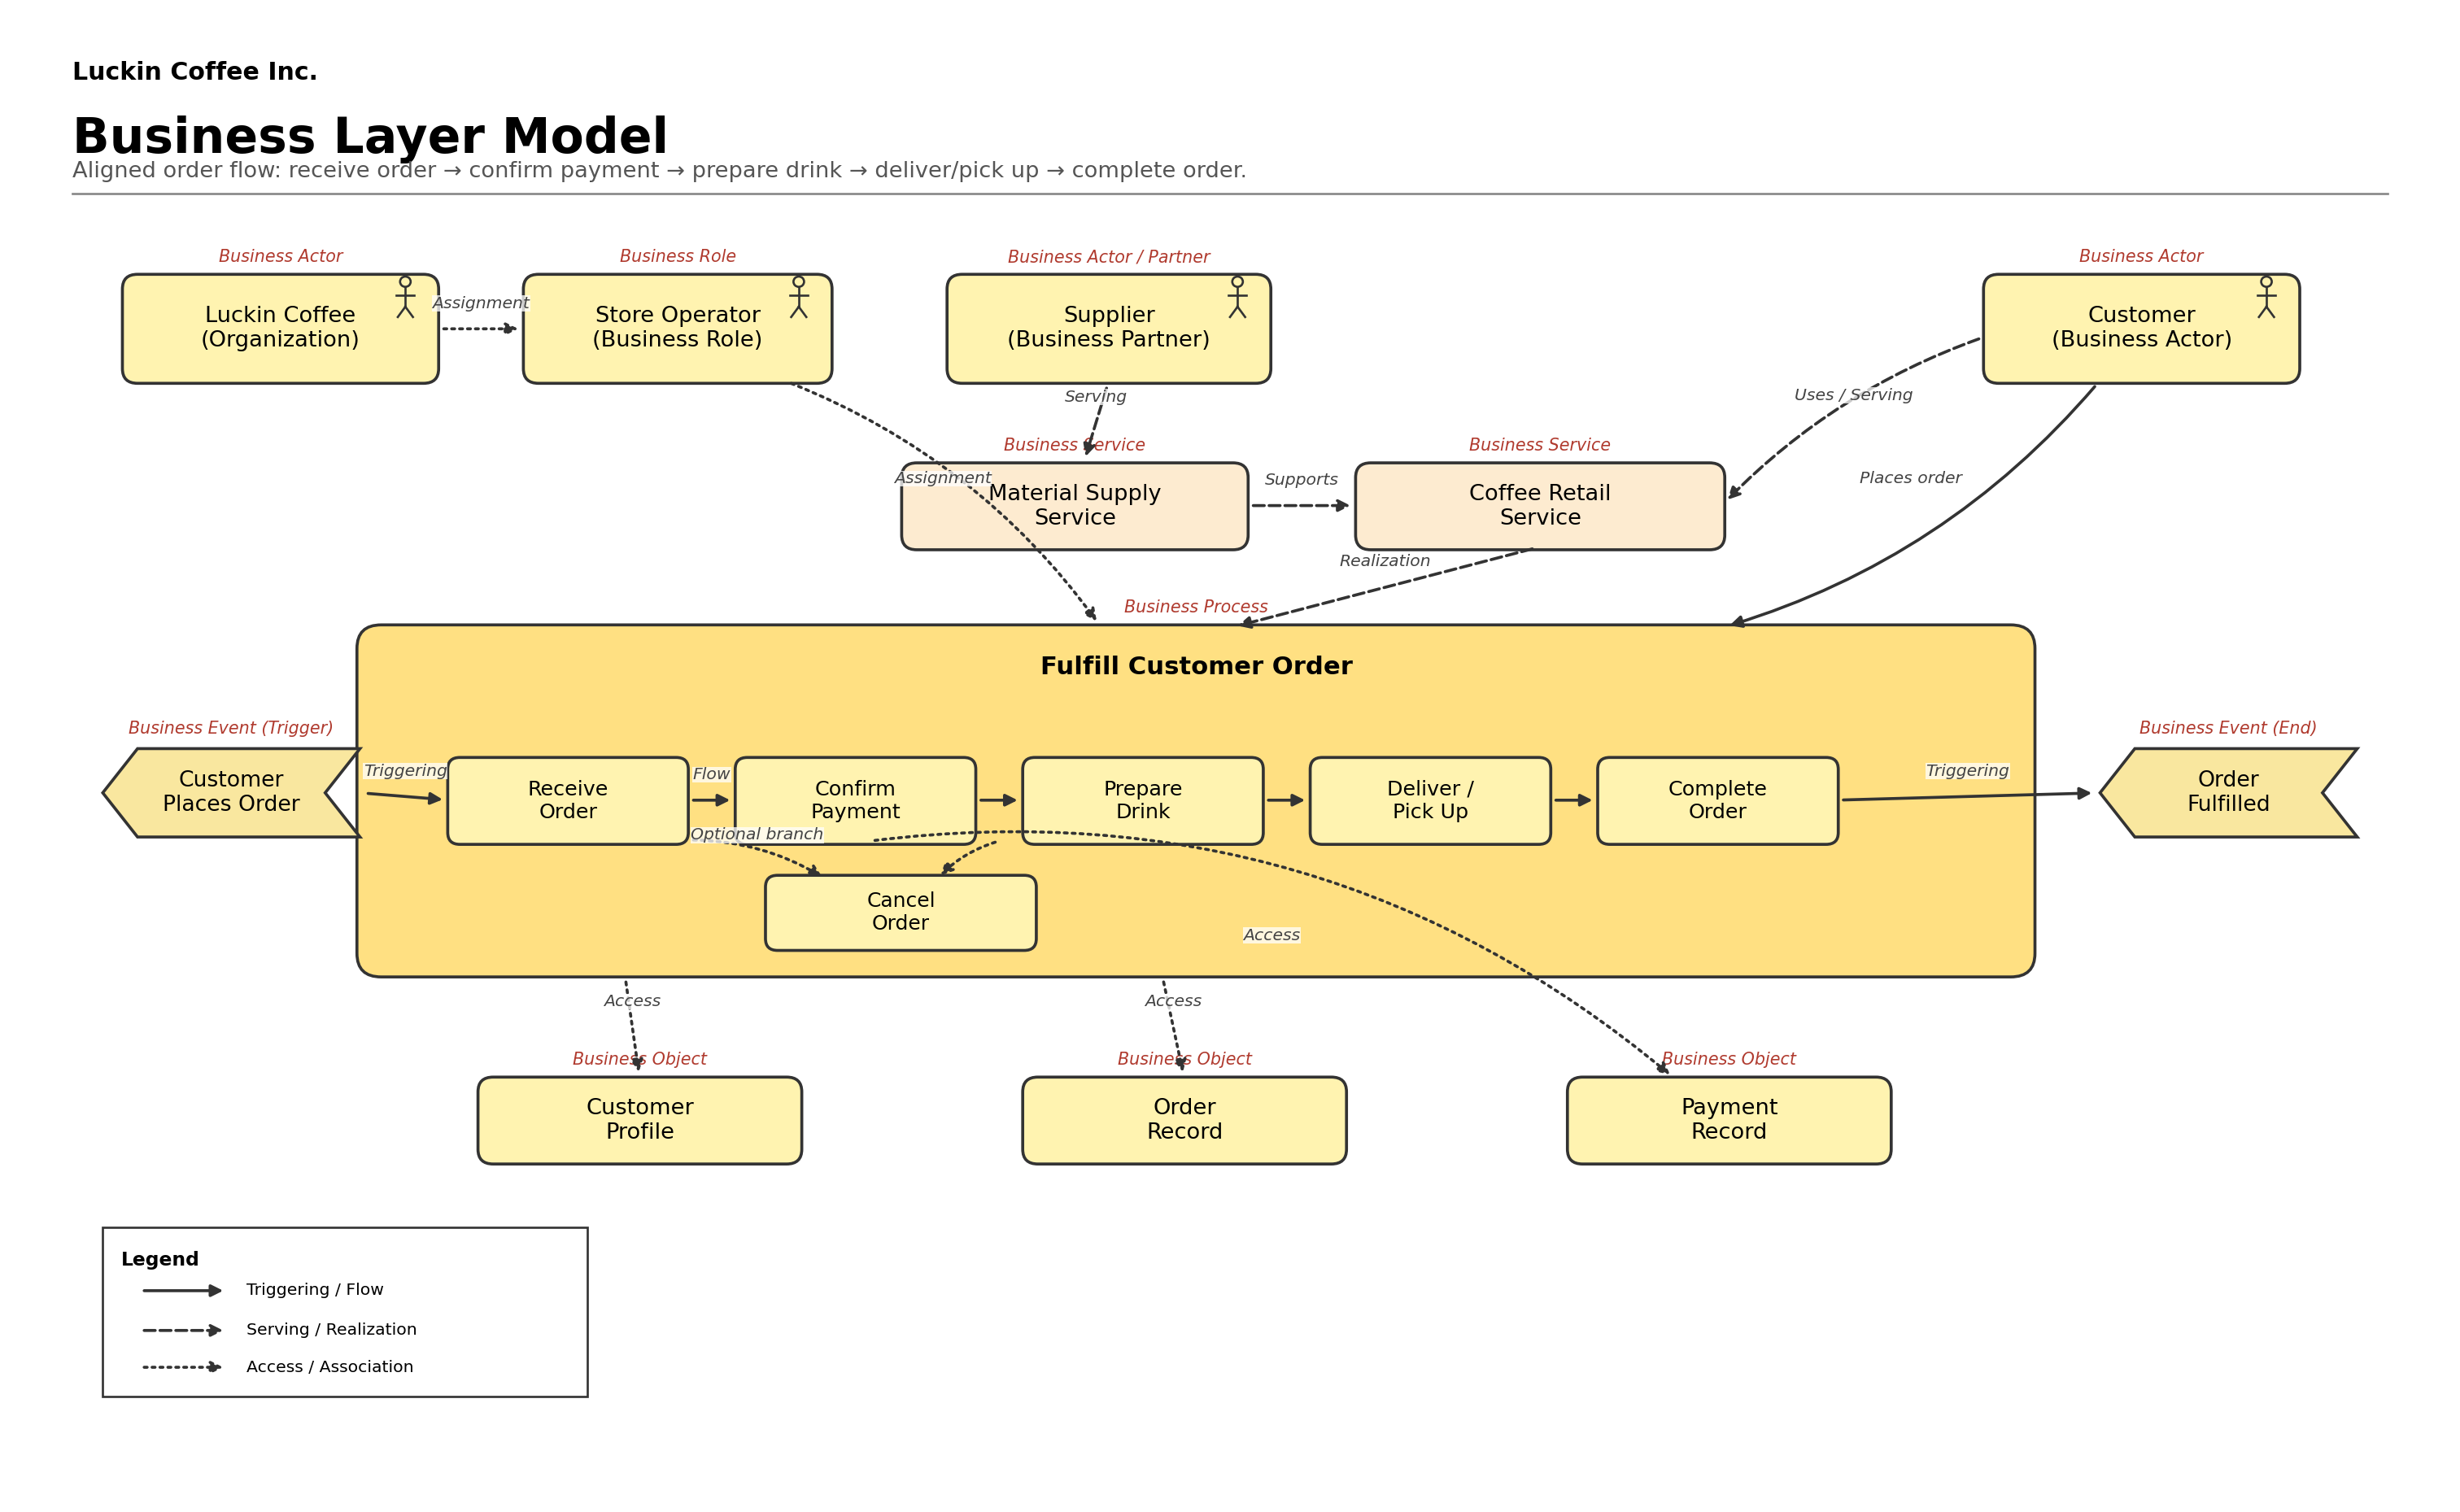
\includegraphics[width=\linewidth,keepaspectratio]{BLM.png}
\caption{Business Layer Model adapted from the Seminar 6 architecture analysis.}
\end{figure}

The model identifies the customer as the external actor, Luckin Coffee as the enterprise actor, store operators and suppliers as key roles, and the Coffee Retail Service as the core business service. The central business process is Fulfill Customer Order, which includes receiving the order, confirming payment, preparing the drink, delivering or handing over the product, and completing the order.

\subsection{Application Layer Model}

The Application Layer Model explains how customer-facing and internal software services support the business process.

\begin{figure}[H]
\centering
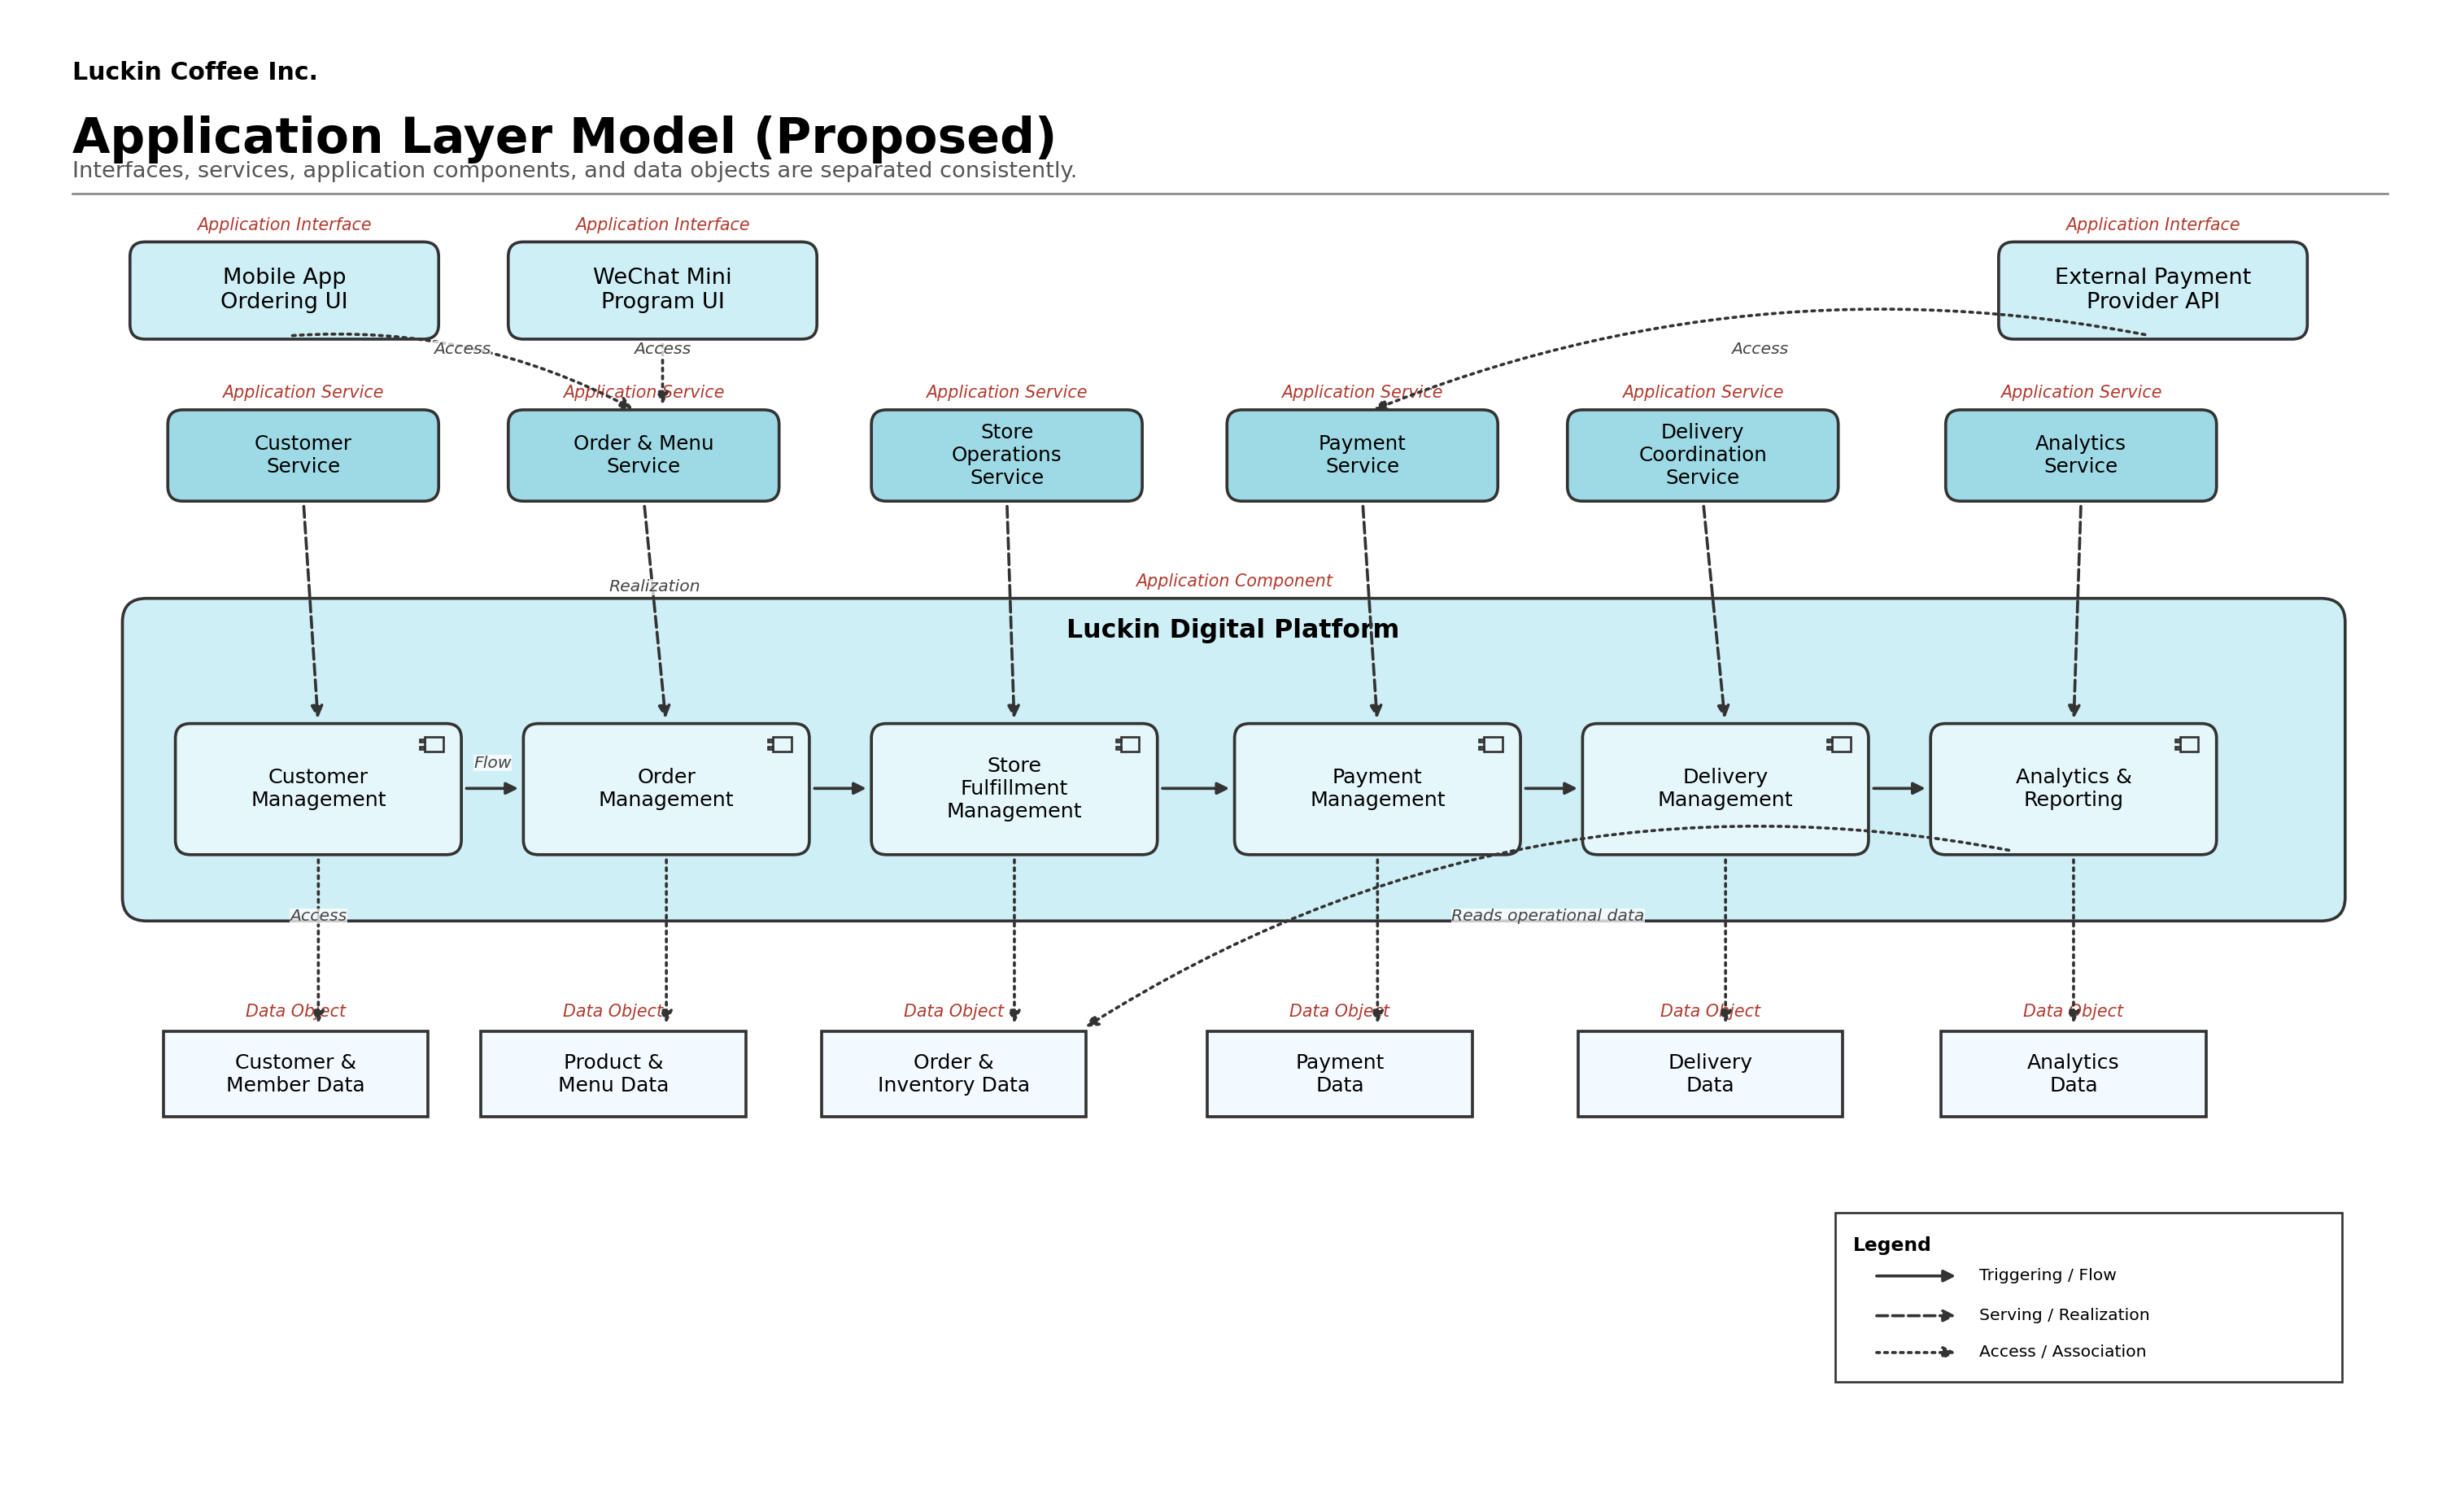
\includegraphics[width=\linewidth,keepaspectratio]{ALM.png}
\caption{Application Layer Model adapted from the Seminar 6 architecture analysis.}
\end{figure}

The key application interfaces are the mobile app and WeChat mini-program. The logical application services include menu browsing, promotion, order management, payment confirmation, fulfilment coordination, customer profile management, inventory support, and analytics. Data objects include customer profiles, orders, products, store information, recipe standards, campaign records, and performance results.

\subsection{Technology Layer Model}

The Technology Layer Model is a proposed architecture view. It should be read as an analytical model, not a confirmed disclosure of Luckin's internal production infrastructure.

\begin{figure}[H]
\centering
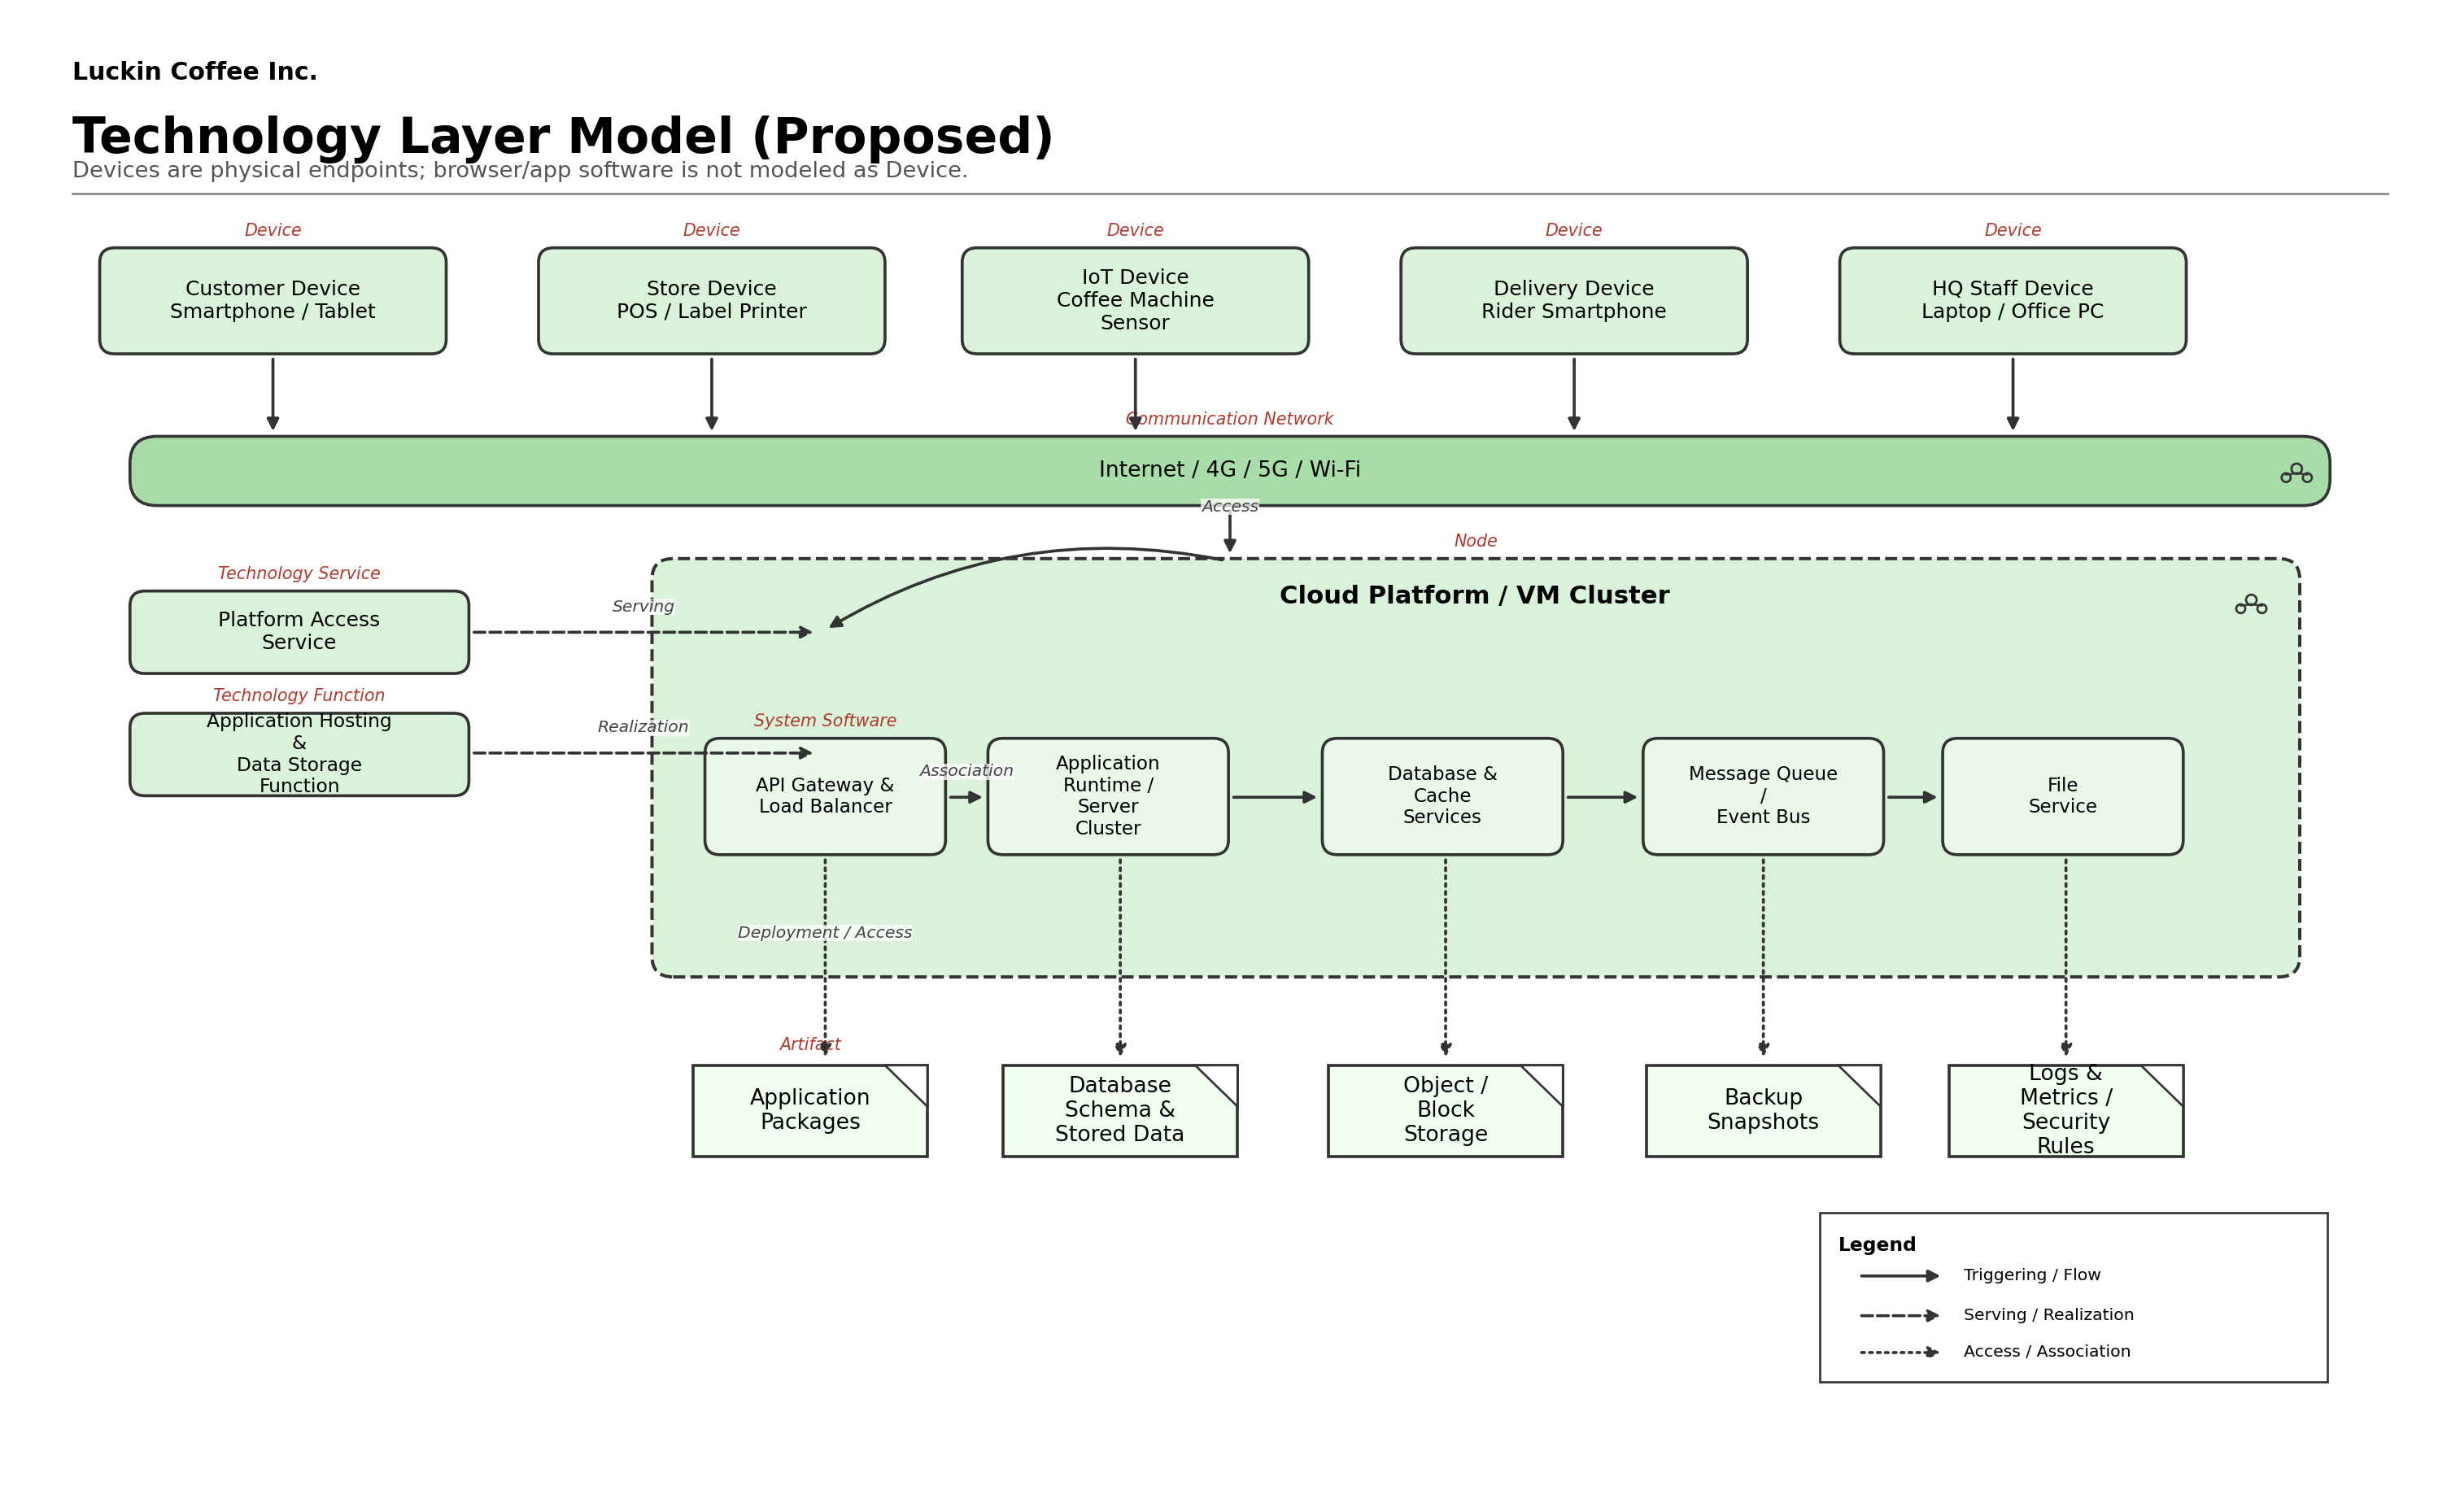
\includegraphics[width=\linewidth,keepaspectratio]{TLM.png}
\caption{Technology Layer Model adapted from the Seminar 6 architecture analysis.}
\end{figure}

This layer includes customer devices, store terminals, network connections, cloud services, databases, monitoring, and integration with external payment and delivery platforms. It is important because Luckin's customer promise depends on low-friction mobile ordering and reliable store fulfilment. If the technology layer fails, the customer-facing service and store process also fail.

% =================== PRESENTATION PLAN ===================
\section{Suggested 10--15 Minute Presentation Plan}

The Seminar 7 instruction sheet says that all group members should present. The following division keeps the talk within 10--15 minutes while allowing each member to own a meaningful part.

\begin{table}[H]
\centering
\small
\caption{Recommended group presentation plan.}
\begin{tabularx}{\textwidth}{P{2.8cm}P{3.1cm}Y}
\toprule
\textbf{Speaker} & \textbf{Time} & \textbf{Content} \\
\midrule
Member 1 & 2 minutes & Introduce Luckin Coffee, mission, vision, products, scale, and why it is suitable for enterprise architecture analysis. \\
Member 2 & 2--3 minutes & Explain business analysis: stakeholders, customers, channels, financial model, internal process, and learning/growth. \\
Member 3 & 3 minutes & Present BSC and Business Model Canvas; connect strategy to objectives, measures, customer value, and revenue/cost structure. \\
Member 4 & 3 minutes & Present EFQM evaluation and main quality-management findings, including strengths and improvement priorities. \\
Member 5 & 3--4 minutes & Present conceptual model, Zachman Row 1, relational data model, and ArchiMate business/application/technology layers. \\
All members & 1 minute & Conclude with the integrated view: Luckin as a digital retail platform whose success depends on alignment between strategy, process, data, applications, and technology. \\
\bottomrule
\end{tabularx}
\end{table}

% =================== CONCLUSION ===================
\section{Conclusion}

Luckin Coffee is an appropriate case for Seminar 7 because its strategy, processes, data, and technology are tightly connected. The company's competitive logic is not based only on selling coffee; it depends on a repeatable operating architecture that links mobile ordering, membership data, standardized store fulfilment, supply-chain resources, partnership stores, analytics, and management control.

The integrated analysis shows that Luckin has strong alignment among the Balanced Scorecard perspectives, Business Model Canvas components, EFQM enablers and results, Zachman Row 1 scope, relational data structures, and ArchiMate layers. Its main strengths are digital customer access, scale, process standardization, product innovation, and measurable operational performance. Its main risks are quality consistency across rapid expansion, delivery cost pressure, employee experience, partner governance, social responsibility, data governance, and system resilience.

Therefore, the recommended enterprise-architecture focus is to maintain growth while strengthening governance and sustainability: keep using data to improve customer value and operational efficiency, but also build stronger mechanisms for trust, people development, partner control, and long-term resilience.

% =================== REFERENCES ===================
\begingroup
\small
\begin{thebibliography}{12}

\bibitem{luckin_ir_overview}
Luckin Coffee Inc. (2026).
\emph{Investor Relations: Company Overview}.
\url{https://investor.lkcoffee.com/}

\bibitem{luckin_fy2025_results}
Luckin Coffee Inc. (2026).
\emph{Luckin Coffee Announces Fourth Quarter and Fiscal Year 2025 Financial Results}.
\url{https://investor.lkcoffee.com/static-files/f6364cc3-1540-4657-b4a9-1c3304de730a}

\bibitem{luckin_q1_2026}
Luckin Coffee Inc. (2026).
\emph{Luckin Coffee Announces First Quarter 2026 Financial Results and Share Repurchase Program}.
\url{https://investor.lkcoffee.com/static-files/3bff7e75-adc7-4d71-bd13-72d8ce7b3416}

\bibitem{luckin_noncoffee_2026}
Luckin Coffee Inc. (2026).
\emph{Luckin Coffee Surpasses RMB20 Billion in Non-Coffee Beverage Sales, Expands Global Store Network Beyond 35,000}.
\url{https://investor.lkcoffee.com/news-releases/news-release-details/luckin-coffee-surpasses-rmb20-billion-non-coffee-beverage-sales}

\bibitem{luckin_annual_reports}
Luckin Coffee Inc. (2026).
\emph{Annual Reports}.
\url{https://investor.lkcoffee.com/financial-information/annual-reports}

\bibitem{efqm}
EFQM. (2025).
\emph{The EFQM Model}.
\url{https://efqm.org/the-efqm-model/}

\bibitem{zachman}
Zachman International. (2025).
\emph{The Zachman Framework}.
\url{https://www.zachman.com/about-the-zachman-framework}

\bibitem{archimate}
The Open Group. (2024).
\emph{ArchiMate Enterprise Architecture Modeling Language}.
\url{https://www.opengroup.org/archimate-forum/archimate-overview}

\end{thebibliography}
\endgroup

\end{document}
